\documentclass[twoside]{book}

% Packages required by doxygen
\usepackage{fixltx2e}
\usepackage{calc}
\usepackage{doxygen}
\usepackage[export]{adjustbox} % also loads graphicx
\usepackage{graphicx}
\usepackage[utf8]{inputenc}
\usepackage{makeidx}
\usepackage{multicol}
\usepackage{multirow}
\PassOptionsToPackage{warn}{textcomp}
\usepackage{textcomp}
\usepackage[nointegrals]{wasysym}
\usepackage[table]{xcolor}

% Font selection
\usepackage[T1]{fontenc}
\usepackage[scaled=.90]{helvet}
\usepackage{courier}
\usepackage{amssymb}
\usepackage{sectsty}
\renewcommand{\familydefault}{\sfdefault}
\allsectionsfont{%
  \fontseries{bc}\selectfont%
  \color{darkgray}%
}
\renewcommand{\DoxyLabelFont}{%
  \fontseries{bc}\selectfont%
  \color{darkgray}%
}
\newcommand{\+}{\discretionary{\mbox{\scriptsize$\hookleftarrow$}}{}{}}

% Page & text layout
\usepackage{geometry}
\geometry{%
  a4paper,%
  top=2.5cm,%
  bottom=2.5cm,%
  left=2.5cm,%
  right=2.5cm%
}
\tolerance=750
\hfuzz=15pt
\hbadness=750
\setlength{\emergencystretch}{15pt}
\setlength{\parindent}{0cm}
\setlength{\parskip}{3ex plus 2ex minus 2ex}
\makeatletter
\renewcommand{\paragraph}{%
  \@startsection{paragraph}{4}{0ex}{-1.0ex}{1.0ex}{%
    \normalfont\normalsize\bfseries\SS@parafont%
  }%
}
\renewcommand{\subparagraph}{%
  \@startsection{subparagraph}{5}{0ex}{-1.0ex}{1.0ex}{%
    \normalfont\normalsize\bfseries\SS@subparafont%
  }%
}
\makeatother

% Headers & footers
\usepackage{fancyhdr}
\pagestyle{fancyplain}
\fancyhead[LE]{\fancyplain{}{\bfseries\thepage}}
\fancyhead[CE]{\fancyplain{}{}}
\fancyhead[RE]{\fancyplain{}{\bfseries\leftmark}}
\fancyhead[LO]{\fancyplain{}{\bfseries\rightmark}}
\fancyhead[CO]{\fancyplain{}{}}
\fancyhead[RO]{\fancyplain{}{\bfseries\thepage}}
\fancyfoot[LE]{\fancyplain{}{}}
\fancyfoot[CE]{\fancyplain{}{}}
\fancyfoot[RE]{\fancyplain{}{\bfseries\scriptsize Generated by Doxygen }}
\fancyfoot[LO]{\fancyplain{}{\bfseries\scriptsize Generated by Doxygen }}
\fancyfoot[CO]{\fancyplain{}{}}
\fancyfoot[RO]{\fancyplain{}{}}
\renewcommand{\footrulewidth}{0.4pt}
\renewcommand{\chaptermark}[1]{%
  \markboth{#1}{}%
}
\renewcommand{\sectionmark}[1]{%
  \markright{\thesection\ #1}%
}

% Indices & bibliography
\usepackage{natbib}
\usepackage[titles]{tocloft}
\setcounter{tocdepth}{3}
\setcounter{secnumdepth}{5}
\makeindex

% Hyperlinks (required, but should be loaded last)
\usepackage{ifpdf}
\ifpdf
  \usepackage[pdftex,pagebackref=true]{hyperref}
\else
  \usepackage[ps2pdf,pagebackref=true]{hyperref}
\fi
\hypersetup{%
  colorlinks=true,%
  linkcolor=blue,%
  citecolor=blue,%
  unicode%
}

% Custom commands
\newcommand{\clearemptydoublepage}{%
  \newpage{\pagestyle{empty}\cleardoublepage}%
}

\usepackage{caption}
\captionsetup{labelsep=space,justification=centering,font={bf},singlelinecheck=off,skip=4pt,position=top}

%===== C O N T E N T S =====

\begin{document}

% Titlepage & ToC
\hypersetup{pageanchor=false,
             bookmarksnumbered=true,
             pdfencoding=unicode
            }
\pagenumbering{alph}
\begin{titlepage}
\vspace*{7cm}
\begin{center}%
{\Large Morpion }\\
\vspace*{1cm}
{\large Generated by Doxygen 1.8.13}\\
\end{center}
\end{titlepage}
\clearemptydoublepage
\pagenumbering{roman}
\tableofcontents
\clearemptydoublepage
\pagenumbering{arabic}
\hypersetup{pageanchor=true}

%--- Begin generated contents ---
\chapter{Namespace Index}
\section{Packages}
Here are the packages with brief descriptions (if available)\+:\begin{DoxyCompactList}
\item\contentsline{section}{\hyperlink{namespace_morpion}{Morpion} }{\pageref{namespace_morpion}}{}
\item\contentsline{section}{\hyperlink{namespace_morpion_1_1_properties}{Morpion.\+Properties} }{\pageref{namespace_morpion_1_1_properties}}{}
\item\contentsline{section}{\hyperlink{namespace_test_morpion}{Test\+Morpion} }{\pageref{namespace_test_morpion}}{}
\end{DoxyCompactList}

\chapter{Hierarchical Index}
\section{Class Hierarchy}
This inheritance list is sorted roughly, but not completely, alphabetically\+:\begin{DoxyCompactList}
\item \contentsline{section}{Morpion.\+Controlor}{\pageref{class_morpion_1_1_controlor}}{}
\item \contentsline{section}{Morpion.\+Data\+Base}{\pageref{class_morpion_1_1_data_base}}{}
\item Form\begin{DoxyCompactList}
\item \contentsline{section}{Morpion.\+View}{\pageref{class_morpion_1_1_view}}{}
\end{DoxyCompactList}
\item \contentsline{section}{Test\+Morpion.\+Game\+Test}{\pageref{class_test_morpion_1_1_game_test}}{}
\item \contentsline{section}{Morpion.\+Model}{\pageref{class_morpion_1_1_model}}{}
\item \contentsline{section}{Morpion.\+Network\+Communication}{\pageref{class_morpion_1_1_network_communication}}{}
\item \contentsline{section}{Test\+Morpion.\+Test\+DB}{\pageref{class_test_morpion_1_1_test_d_b}}{}
\end{DoxyCompactList}

\chapter{Class Index}
\section{Class List}
Here are the classes, structs, unions and interfaces with brief descriptions\+:\begin{DoxyCompactList}
\item\contentsline{section}{\hyperlink{class_morpion_1_1_controlor}{Morpion.\+Controlor} }{\pageref{class_morpion_1_1_controlor}}{}
\item\contentsline{section}{\hyperlink{class_morpion_1_1_data_base}{Morpion.\+Data\+Base} \\*The class give access to DB }{\pageref{class_morpion_1_1_data_base}}{}
\item\contentsline{section}{\hyperlink{class_test_morpion_1_1_game_test}{Test\+Morpion.\+Game\+Test} }{\pageref{class_test_morpion_1_1_game_test}}{}
\item\contentsline{section}{\hyperlink{class_morpion_1_1_model}{Morpion.\+Model} \\*}{\pageref{class_morpion_1_1_model}}{}
\item\contentsline{section}{\hyperlink{class_morpion_1_1_network_communication}{Morpion.\+Network\+Communication} }{\pageref{class_morpion_1_1_network_communication}}{}
\item\contentsline{section}{\hyperlink{class_test_morpion_1_1_test_d_b}{Test\+Morpion.\+Test\+DB} }{\pageref{class_test_morpion_1_1_test_d_b}}{}
\item\contentsline{section}{\hyperlink{class_morpion_1_1_view}{Morpion.\+View} \\*Form view, allows the display of the different interfaces }{\pageref{class_morpion_1_1_view}}{}
\end{DoxyCompactList}

\chapter{File Index}
\section{File List}
Here is a list of all files with brief descriptions\+:\begin{DoxyCompactList}
\item\contentsline{section}{C\+O\+D\+E/\+Morpion/\+Morpion/\hyperlink{_controlor_8cs}{Controlor.\+cs} }{\pageref{_controlor_8cs}}{}
\item\contentsline{section}{C\+O\+D\+E/\+Morpion/\+Morpion/\hyperlink{_data_base_8cs}{Data\+Base.\+cs} }{\pageref{_data_base_8cs}}{}
\item\contentsline{section}{C\+O\+D\+E/\+Morpion/\+Morpion/\hyperlink{_model_8cs}{Model.\+cs} }{\pageref{_model_8cs}}{}
\item\contentsline{section}{C\+O\+D\+E/\+Morpion/\+Morpion/\hyperlink{_network_communication_8cs}{Network\+Communication.\+cs} }{\pageref{_network_communication_8cs}}{}
\item\contentsline{section}{C\+O\+D\+E/\+Morpion/\+Morpion/\hyperlink{_program_8cs}{Program.\+cs} }{\pageref{_program_8cs}}{}
\item\contentsline{section}{C\+O\+D\+E/\+Morpion/\+Morpion/\hyperlink{_view_8cs}{View.\+cs} }{\pageref{_view_8cs}}{}
\item\contentsline{section}{C\+O\+D\+E/\+Morpion/\+Morpion/\hyperlink{_view_8_designer_8cs}{View.\+Designer.\+cs} }{\pageref{_view_8_designer_8cs}}{}
\item\contentsline{section}{C\+O\+D\+E/\+Morpion/\+Morpion/obj/\+Debug/\hyperlink{_morpion_2obj_2_debug_2_temporary_generated_file__036_c0_b5_b-1481-4323-8_d20-8_f5_a_d_c_b23_d92_8cs}{Temporary\+Generated\+File\+\_\+036\+C0\+B5\+B-\/1481-\/4323-\/8\+D20-\/8\+F5\+A\+D\+C\+B23\+D92.\+cs} }{\pageref{_morpion_2obj_2_debug_2_temporary_generated_file__036_c0_b5_b-1481-4323-8_d20-8_f5_a_d_c_b23_d92_8cs}}{}
\item\contentsline{section}{C\+O\+D\+E/\+Morpion/\+Morpion/obj/\+Debug/\hyperlink{_morpion_2obj_2_debug_2_temporary_generated_file__5937a670-0e60-4077-877b-f7221da3dda1_8cs}{Temporary\+Generated\+File\+\_\+5937a670-\/0e60-\/4077-\/877b-\/f7221da3dda1.\+cs} }{\pageref{_morpion_2obj_2_debug_2_temporary_generated_file__5937a670-0e60-4077-877b-f7221da3dda1_8cs}}{}
\item\contentsline{section}{C\+O\+D\+E/\+Morpion/\+Morpion/obj/\+Debug/\hyperlink{_morpion_2obj_2_debug_2_temporary_generated_file___e7_a71_f73-0_f8_d-4_b9_b-_b56_e-8_e70_b10_b_c5_d3_8cs}{Temporary\+Generated\+File\+\_\+\+E7\+A71\+F73-\/0\+F8\+D-\/4\+B9\+B-\/\+B56\+E-\/8\+E70\+B10\+B\+C5\+D3.\+cs} }{\pageref{_morpion_2obj_2_debug_2_temporary_generated_file___e7_a71_f73-0_f8_d-4_b9_b-_b56_e-8_e70_b10_b_c5_d3_8cs}}{}
\item\contentsline{section}{C\+O\+D\+E/\+Morpion/\+Morpion/\+Properties/\hyperlink{_morpion_2_properties_2_assembly_info_8cs}{Assembly\+Info.\+cs} }{\pageref{_morpion_2_properties_2_assembly_info_8cs}}{}
\item\contentsline{section}{C\+O\+D\+E/\+Morpion/\+Morpion/\+Properties/\hyperlink{_resources_8_designer_8cs}{Resources.\+Designer.\+cs} }{\pageref{_resources_8_designer_8cs}}{}
\item\contentsline{section}{C\+O\+D\+E/\+Morpion/\+Morpion/\+Properties/\hyperlink{_settings_8_designer_8cs}{Settings.\+Designer.\+cs} }{\pageref{_settings_8_designer_8cs}}{}
\item\contentsline{section}{C\+O\+D\+E/\+Morpion/\+Test\+Morpion/\hyperlink{game_test_8cs}{game\+Test.\+cs} }{\pageref{game_test_8cs}}{}
\item\contentsline{section}{C\+O\+D\+E/\+Morpion/\+Test\+Morpion/\hyperlink{_test_d_b_8cs}{Test\+D\+B.\+cs} }{\pageref{_test_d_b_8cs}}{}
\item\contentsline{section}{C\+O\+D\+E/\+Morpion/\+Test\+Morpion/obj/\+Debug/\hyperlink{_test_morpion_2obj_2_debug_2_temporary_generated_file__036_c0_b5_b-1481-4323-8_d20-8_f5_a_d_c_b23_d92_8cs}{Temporary\+Generated\+File\+\_\+036\+C0\+B5\+B-\/1481-\/4323-\/8\+D20-\/8\+F5\+A\+D\+C\+B23\+D92.\+cs} }{\pageref{_test_morpion_2obj_2_debug_2_temporary_generated_file__036_c0_b5_b-1481-4323-8_d20-8_f5_a_d_c_b23_d92_8cs}}{}
\item\contentsline{section}{C\+O\+D\+E/\+Morpion/\+Test\+Morpion/obj/\+Debug/\hyperlink{_test_morpion_2obj_2_debug_2_temporary_generated_file__5937a670-0e60-4077-877b-f7221da3dda1_8cs}{Temporary\+Generated\+File\+\_\+5937a670-\/0e60-\/4077-\/877b-\/f7221da3dda1.\+cs} }{\pageref{_test_morpion_2obj_2_debug_2_temporary_generated_file__5937a670-0e60-4077-877b-f7221da3dda1_8cs}}{}
\item\contentsline{section}{C\+O\+D\+E/\+Morpion/\+Test\+Morpion/obj/\+Debug/\hyperlink{_test_morpion_2obj_2_debug_2_temporary_generated_file___e7_a71_f73-0_f8_d-4_b9_b-_b56_e-8_e70_b10_b_c5_d3_8cs}{Temporary\+Generated\+File\+\_\+\+E7\+A71\+F73-\/0\+F8\+D-\/4\+B9\+B-\/\+B56\+E-\/8\+E70\+B10\+B\+C5\+D3.\+cs} }{\pageref{_test_morpion_2obj_2_debug_2_temporary_generated_file___e7_a71_f73-0_f8_d-4_b9_b-_b56_e-8_e70_b10_b_c5_d3_8cs}}{}
\item\contentsline{section}{C\+O\+D\+E/\+Morpion/\+Test\+Morpion/\+Properties/\hyperlink{_test_morpion_2_properties_2_assembly_info_8cs}{Assembly\+Info.\+cs} }{\pageref{_test_morpion_2_properties_2_assembly_info_8cs}}{}
\end{DoxyCompactList}

\chapter{Namespace Documentation}
\hypertarget{namespace_morpion}{}\section{Morpion Namespace Reference}
\label{namespace_morpion}\index{Morpion@{Morpion}}
\subsection*{Namespaces}
\begin{DoxyCompactItemize}
\item 
namespace \hyperlink{namespace_morpion_1_1_properties}{Properties}
\end{DoxyCompactItemize}
\subsection*{Classes}
\begin{DoxyCompactItemize}
\item 
class \hyperlink{class_morpion_1_1_controlor}{Controlor}
\begin{DoxyCompactList}\small\item\em \hyperlink{class_morpion_1_1_controlor}{Controlor} manage the application. To access data, controlor call model and ask specific data. when it has data, he send to view. \end{DoxyCompactList}\item 
class \hyperlink{class_morpion_1_1_data_base}{Data\+Base}
\begin{DoxyCompactList}\small\item\em The class give access to DB \end{DoxyCompactList}\item 
class \hyperlink{class_morpion_1_1_model}{Model}
\begin{DoxyCompactList}\small\item\em containt all data of the game and sends the required data to control \end{DoxyCompactList}\item 
class \hyperlink{class_morpion_1_1_network_communication}{Network\+Communication}
\item 
class {\bfseries Program}
\item 
class \hyperlink{class_morpion_1_1score}{score}
\begin{DoxyCompactList}\small\item\em this class allows to create an object containing the score between 2 players \end{DoxyCompactList}\item 
class \hyperlink{class_morpion_1_1_view}{View}
\begin{DoxyCompactList}\small\item\em The form Contain all views of game \end{DoxyCompactList}\end{DoxyCompactItemize}

\hypertarget{namespace_morpion_1_1_properties}{}\section{Morpion.\+Properties Namespace Reference}
\label{namespace_morpion_1_1_properties}\index{Morpion.\+Properties@{Morpion.\+Properties}}
\subsection*{Classes}
\begin{DoxyCompactItemize}
\item 
class {\bfseries Resources}
\begin{DoxyCompactList}\small\item\em A strongly-\/typed resource class, for looking up localized strings, etc. \end{DoxyCompactList}\item 
class {\bfseries Settings}
\end{DoxyCompactItemize}

\hypertarget{namespace_test_morpion}{}\section{Test\+Morpion Namespace Reference}
\label{namespace_test_morpion}\index{Test\+Morpion@{Test\+Morpion}}
\subsection*{Classes}
\begin{DoxyCompactItemize}
\item 
class \hyperlink{class_test_morpion_1_1_game_test}{Game\+Test}
\item 
class \hyperlink{class_test_morpion_1_1_test_d_b}{Test\+DB}
\end{DoxyCompactItemize}

\chapter{Class Documentation}
\hypertarget{class_morpion_1_1_controlor}{}\section{Morpion.\+Controlor Class Reference}
\label{class_morpion_1_1_controlor}\index{Morpion.\+Controlor@{Morpion.\+Controlor}}


\hyperlink{class_morpion_1_1_controlor}{Controlor} manage the application. To access data, controlor call model and ask specific data. when it has data, he send to view.  


\subsection*{Public Member Functions}
\begin{DoxyCompactItemize}
\item 
\hyperlink{class_morpion_1_1_controlor_ac43833b173f2a2e53cab4dd277d6fc0f}{Controlor} ()
\begin{DoxyCompactList}\small\item\em Constructor of control, he call model and ask all data before to execute program \end{DoxyCompactList}\end{DoxyCompactItemize}


\subsection{Detailed Description}
\hyperlink{class_morpion_1_1_controlor}{Controlor} manage the application. To access data, controlor call model and ask specific data. when it has data, he send to view. 



\subsection{Constructor \& Destructor Documentation}
\mbox{\Hypertarget{class_morpion_1_1_controlor_ac43833b173f2a2e53cab4dd277d6fc0f}\label{class_morpion_1_1_controlor_ac43833b173f2a2e53cab4dd277d6fc0f}} 
\index{Morpion\+::\+Controlor@{Morpion\+::\+Controlor}!Controlor@{Controlor}}
\index{Controlor@{Controlor}!Morpion\+::\+Controlor@{Morpion\+::\+Controlor}}
\subsubsection{\texorpdfstring{Controlor()}{Controlor()}}
{\footnotesize\ttfamily Morpion.\+Controlor.\+Controlor (\begin{DoxyParamCaption}{ }\end{DoxyParamCaption})}



Constructor of control, he call model and ask all data before to execute program 



The documentation for this class was generated from the following file\+:\begin{DoxyCompactItemize}
\item 
C\+:/\+Users/\+Diogo.\+V\+I\+E\+I\+R\+A-\/\+F\+E\+R\+R\+E\+I\+R/\+One\+Drive -\/ C\+P\+N\+V/pre-\/tpi/\+Morpion\+\_\+\+Pre-\/\+T\+P\+I/\+C\+O\+D\+E/\+Morpion/\+Morpion/\hyperlink{_controlor_8cs}{Controlor.\+cs}\end{DoxyCompactItemize}

\hypertarget{class_morpion_1_1_data_base}{}\section{Morpion.\+Data\+Base Class Reference}
\label{class_morpion_1_1_data_base}\index{Morpion.\+Data\+Base@{Morpion.\+Data\+Base}}


The class give access to DB  


\subsection*{Public Member Functions}
\begin{DoxyCompactItemize}
\item 
\hyperlink{class_morpion_1_1_data_base_a0d69b39dbf424f7d4105df7a3ec0a586}{Data\+Base} (string db\+Name)
\begin{DoxyCompactList}\small\item\em Create Database and table scores \end{DoxyCompactList}\item 
void \hyperlink{class_morpion_1_1_data_base_a08b6bf1e688f66fbde3e818e08503be6}{Clear\+Scores} ()
\begin{DoxyCompactList}\small\item\em clear all scores \end{DoxyCompactList}\item 
void \hyperlink{class_morpion_1_1_data_base_ac964919b18e41d29326dd96ff9694d5a}{Insert\+Score} (string user\+Name01, string user\+Name02, int score01, int score02)
\begin{DoxyCompactList}\small\item\em Add column in database with param values \end{DoxyCompactList}\item 
List$<$ string $>$ \hyperlink{class_morpion_1_1_data_base_a45bfe0e1b60c377da0b085cb2590b7bf}{Score\+List} ()
\begin{DoxyCompactList}\small\item\em Select all scores in db and send a list with them \end{DoxyCompactList}\end{DoxyCompactItemize}
\subsection*{Properties}
\begin{DoxyCompactItemize}
\item 
int \hyperlink{class_morpion_1_1_data_base_ac0104fe497ec69fc184498e3e904b41f}{limit}\hspace{0.3cm}{\ttfamily  \mbox{[}get, set\mbox{]}}
\begin{DoxyCompactList}\small\item\em get or set limit values in db \end{DoxyCompactList}\end{DoxyCompactItemize}


\subsection{Detailed Description}
The class give access to DB 



\subsection{Constructor \& Destructor Documentation}
\mbox{\Hypertarget{class_morpion_1_1_data_base_a0d69b39dbf424f7d4105df7a3ec0a586}\label{class_morpion_1_1_data_base_a0d69b39dbf424f7d4105df7a3ec0a586}} 
\index{Morpion\+::\+Data\+Base@{Morpion\+::\+Data\+Base}!Data\+Base@{Data\+Base}}
\index{Data\+Base@{Data\+Base}!Morpion\+::\+Data\+Base@{Morpion\+::\+Data\+Base}}
\subsubsection{\texorpdfstring{Data\+Base()}{DataBase()}}
{\footnotesize\ttfamily Morpion.\+Data\+Base.\+Data\+Base (\begin{DoxyParamCaption}\item[{string}]{db\+Name }\end{DoxyParamCaption})}



Create Database and table scores 


\begin{DoxyParams}{Parameters}
{\em db\+Name} & name of Database\\
\hline
\end{DoxyParams}


\subsection{Member Function Documentation}
\mbox{\Hypertarget{class_morpion_1_1_data_base_a08b6bf1e688f66fbde3e818e08503be6}\label{class_morpion_1_1_data_base_a08b6bf1e688f66fbde3e818e08503be6}} 
\index{Morpion\+::\+Data\+Base@{Morpion\+::\+Data\+Base}!Clear\+Scores@{Clear\+Scores}}
\index{Clear\+Scores@{Clear\+Scores}!Morpion\+::\+Data\+Base@{Morpion\+::\+Data\+Base}}
\subsubsection{\texorpdfstring{Clear\+Scores()}{ClearScores()}}
{\footnotesize\ttfamily void Morpion.\+Data\+Base.\+Clear\+Scores (\begin{DoxyParamCaption}{ }\end{DoxyParamCaption})}



clear all scores 

\mbox{\Hypertarget{class_morpion_1_1_data_base_ac964919b18e41d29326dd96ff9694d5a}\label{class_morpion_1_1_data_base_ac964919b18e41d29326dd96ff9694d5a}} 
\index{Morpion\+::\+Data\+Base@{Morpion\+::\+Data\+Base}!Insert\+Score@{Insert\+Score}}
\index{Insert\+Score@{Insert\+Score}!Morpion\+::\+Data\+Base@{Morpion\+::\+Data\+Base}}
\subsubsection{\texorpdfstring{Insert\+Score()}{InsertScore()}}
{\footnotesize\ttfamily void Morpion.\+Data\+Base.\+Insert\+Score (\begin{DoxyParamCaption}\item[{string}]{user\+Name01,  }\item[{string}]{user\+Name02,  }\item[{int}]{score01,  }\item[{int}]{score02 }\end{DoxyParamCaption})}



Add column in database with param values 


\begin{DoxyParams}{Parameters}
{\em user\+Name01} & name of first user\\
\hline
{\em user\+Name02} & name of second user\\
\hline
{\em score01} & score of first user\\
\hline
{\em score02} & score of second user\\
\hline
\end{DoxyParams}
\mbox{\Hypertarget{class_morpion_1_1_data_base_a45bfe0e1b60c377da0b085cb2590b7bf}\label{class_morpion_1_1_data_base_a45bfe0e1b60c377da0b085cb2590b7bf}} 
\index{Morpion\+::\+Data\+Base@{Morpion\+::\+Data\+Base}!Score\+List@{Score\+List}}
\index{Score\+List@{Score\+List}!Morpion\+::\+Data\+Base@{Morpion\+::\+Data\+Base}}
\subsubsection{\texorpdfstring{Score\+List()}{ScoreList()}}
{\footnotesize\ttfamily List$<$string$>$ Morpion.\+Data\+Base.\+Score\+List (\begin{DoxyParamCaption}{ }\end{DoxyParamCaption})}



Select all scores in db and send a list with them 

\begin{DoxyReturn}{Returns}
list with all scores
\end{DoxyReturn}


\subsection{Property Documentation}
\mbox{\Hypertarget{class_morpion_1_1_data_base_ac0104fe497ec69fc184498e3e904b41f}\label{class_morpion_1_1_data_base_ac0104fe497ec69fc184498e3e904b41f}} 
\index{Morpion\+::\+Data\+Base@{Morpion\+::\+Data\+Base}!limit@{limit}}
\index{limit@{limit}!Morpion\+::\+Data\+Base@{Morpion\+::\+Data\+Base}}
\subsubsection{\texorpdfstring{limit}{limit}}
{\footnotesize\ttfamily int Morpion.\+Data\+Base.\+limit\hspace{0.3cm}{\ttfamily [get]}, {\ttfamily [set]}}



get or set limit values in db 



The documentation for this class was generated from the following file\+:\begin{DoxyCompactItemize}
\item 
C\+O\+D\+E/\+Morpion/\+Morpion/\hyperlink{_data_base_8cs}{Data\+Base.\+cs}\end{DoxyCompactItemize}

\hypertarget{class_morpion_1_1_model}{}\section{Morpion.\+Model Class Reference}
\label{class_morpion_1_1_model}\index{Morpion.\+Model@{Morpion.\+Model}}


containt all data of the game and sends the required data to control  


\subsection*{Public Member Functions}
\begin{DoxyCompactItemize}
\item 
\hyperlink{class_morpion_1_1_model_a459b4901421170316a320d2e7d6408b4}{Model} ()
\begin{DoxyCompactList}\small\item\em constructor of model\textquotesingle{}s class \end{DoxyCompactList}\item 
bool \hyperlink{class_morpion_1_1_model_a76f2eb1ec20a4aa78cca17514a0b94e1}{Check\+Game} (int id)
\begin{DoxyCompactList}\small\item\em Check state of game when user put the last our symbol, return true value when equality an exception are generate \end{DoxyCompactList}\item 
int \hyperlink{class_morpion_1_1_model_a02dd1ba77ebd6563c86164592b339ed0}{AI} (int lvl)
\begin{DoxyCompactList}\small\item\em generate AI to play with user \end{DoxyCompactList}\item 
void \hyperlink{class_morpion_1_1_model_af97f1128b5beaa34f151304c84ee1a80}{Save\+Game} ()
\begin{DoxyCompactList}\small\item\em save score of player(s) in db \end{DoxyCompactList}\item 
void \hyperlink{class_morpion_1_1_model_ab5dee79623ee37ae8ccb63bade900dcf}{Clear\+DB} ()
\begin{DoxyCompactList}\small\item\em delete all scores in db \end{DoxyCompactList}\end{DoxyCompactItemize}
\subsection*{Properties}
\begin{DoxyCompactItemize}
\item 
List$<$ \hyperlink{class_morpion_1_1score}{score} $>$ \hyperlink{class_morpion_1_1_model_a088eacfea472a460a1b6ec1e85f3bc8a}{Get\+Score}\hspace{0.3cm}{\ttfamily  \mbox{[}get\mbox{]}}
\begin{DoxyCompactList}\small\item\em send all records on database \end{DoxyCompactList}\item 
bool \hyperlink{class_morpion_1_1_model_a47fdf7d505cd7dd8f43b73bd7ac2feb4}{Multi}\hspace{0.3cm}{\ttfamily  \mbox{[}get, set\mbox{]}}
\begin{DoxyCompactList}\small\item\em \+\_\+multi\textquotesingle{}s accessor it\textquotesingle{}s a multiplayer game? \end{DoxyCompactList}\item 
string \hyperlink{class_morpion_1_1_model_a95982016831a025998f12b630550d009}{Name\+P1}\hspace{0.3cm}{\ttfamily  \mbox{[}get, set\mbox{]}}
\begin{DoxyCompactList}\small\item\em \+\_\+name\+P1\textquotesingle{}s accessor get or set name of player 02 \end{DoxyCompactList}\item 
int \hyperlink{class_morpion_1_1_model_ac07840451cf10dfa2bff76768425963b}{Score\+P1}\hspace{0.3cm}{\ttfamily  \mbox{[}get, set\mbox{]}}
\begin{DoxyCompactList}\small\item\em \+\_\+score\+P1\textquotesingle{}s accessor get or set score of player 01 \end{DoxyCompactList}\item 
string \hyperlink{class_morpion_1_1_model_a54eefe46fd6d10d15f8b34cf2ee943e6}{Name\+P2}\hspace{0.3cm}{\ttfamily  \mbox{[}get, set\mbox{]}}
\begin{DoxyCompactList}\small\item\em \+\_\+name\+P2\textquotesingle{}s accessor get or set name of player 02 \end{DoxyCompactList}\item 
string \hyperlink{class_morpion_1_1_model_adc7a7e85bab1d3a90418792a1e8078cf}{Actual\+Player}\hspace{0.3cm}{\ttfamily  \mbox{[}get\mbox{]}}
\begin{DoxyCompactList}\small\item\em get name current player \end{DoxyCompactList}\item 
int \hyperlink{class_morpion_1_1_model_a5c9fac9656289625158e863d2b7850ff}{Score\+P2}\hspace{0.3cm}{\ttfamily  \mbox{[}get, set\mbox{]}}
\begin{DoxyCompactList}\small\item\em \+\_\+score\+P2\textquotesingle{}s accessor get or set score of player 02 \end{DoxyCompactList}\item 
\hyperlink{class_morpion_1_1_view}{View} \hyperlink{class_morpion_1_1_model_a9e23eaa776d26da2b6ef98aa5fb8db88}{View}\hspace{0.3cm}{\ttfamily  \mbox{[}set\mbox{]}}
\begin{DoxyCompactList}\small\item\em \+\_\+view\textquotesingle{}s accessor \end{DoxyCompactList}\item 
int \mbox{[}$\,$\mbox{]} \hyperlink{class_morpion_1_1_model_a565b0372c7f7833b244c03721f7eebd6}{Game\+Array}\hspace{0.3cm}{\ttfamily  \mbox{[}get, set\mbox{]}}
\begin{DoxyCompactList}\small\item\em \+\_\+game\+Array\textquotesingle{}s accessor get or set the plateform\textquotesingle{}s game \end{DoxyCompactList}\item 
int \hyperlink{class_morpion_1_1_model_a56f84098c9bde669925d9a6850aaf061}{What\+Player}\hspace{0.3cm}{\ttfamily  \mbox{[}get, set\mbox{]}}
\begin{DoxyCompactList}\small\item\em \+\_\+waht\+Player\textquotesingle{}s accessor return number of player, 1 or 2 \end{DoxyCompactList}\item 
int \hyperlink{class_morpion_1_1_model_a9a111fd09fe1b8cfd2beada02951f6fa}{Db\+Limit}\hspace{0.3cm}{\ttfamily  \mbox{[}set\mbox{]}}
\begin{DoxyCompactList}\small\item\em define limit of scores in db \end{DoxyCompactList}\item 
int \hyperlink{class_morpion_1_1_model_a99d714c546cbe2f67a4cdb04c0c32f1f}{Lvl\+AI}\hspace{0.3cm}{\ttfamily  \mbox{[}get, set\mbox{]}}
\begin{DoxyCompactList}\small\item\em define the level of AI (Artificial Intelligence) \end{DoxyCompactList}\end{DoxyCompactItemize}


\subsection{Detailed Description}
containt all data of the game and sends the required data to control 



\subsection{Constructor \& Destructor Documentation}
\mbox{\Hypertarget{class_morpion_1_1_model_a459b4901421170316a320d2e7d6408b4}\label{class_morpion_1_1_model_a459b4901421170316a320d2e7d6408b4}} 
\index{Morpion\+::\+Model@{Morpion\+::\+Model}!Model@{Model}}
\index{Model@{Model}!Morpion\+::\+Model@{Morpion\+::\+Model}}
\subsubsection{\texorpdfstring{Model()}{Model()}}
{\footnotesize\ttfamily Morpion.\+Model.\+Model (\begin{DoxyParamCaption}{ }\end{DoxyParamCaption})}



constructor of model\textquotesingle{}s class 



\subsection{Member Function Documentation}
\mbox{\Hypertarget{class_morpion_1_1_model_a02dd1ba77ebd6563c86164592b339ed0}\label{class_morpion_1_1_model_a02dd1ba77ebd6563c86164592b339ed0}} 
\index{Morpion\+::\+Model@{Morpion\+::\+Model}!AI@{AI}}
\index{AI@{AI}!Morpion\+::\+Model@{Morpion\+::\+Model}}
\subsubsection{\texorpdfstring{A\+I()}{AI()}}
{\footnotesize\ttfamily int Morpion.\+Model.\+AI (\begin{DoxyParamCaption}\item[{int}]{lvl }\end{DoxyParamCaption})}



generate AI to play with user 


\begin{DoxyParams}{Parameters}
{\em lvl} & insert the difficult of AI. 1 easy, 2 medium, 3 hard\\
\hline
\end{DoxyParams}
\mbox{\Hypertarget{class_morpion_1_1_model_a76f2eb1ec20a4aa78cca17514a0b94e1}\label{class_morpion_1_1_model_a76f2eb1ec20a4aa78cca17514a0b94e1}} 
\index{Morpion\+::\+Model@{Morpion\+::\+Model}!Check\+Game@{Check\+Game}}
\index{Check\+Game@{Check\+Game}!Morpion\+::\+Model@{Morpion\+::\+Model}}
\subsubsection{\texorpdfstring{Check\+Game()}{CheckGame()}}
{\footnotesize\ttfamily bool Morpion.\+Model.\+Check\+Game (\begin{DoxyParamCaption}\item[{int}]{id }\end{DoxyParamCaption})}



Check state of game when user put the last our symbol, return true value when equality an exception are generate 


\begin{DoxyParams}{Parameters}
{\em id} & match a location where player have place his symbol in game array\\
\hline
\end{DoxyParams}
\begin{DoxyReturn}{Returns}

\end{DoxyReturn}
\mbox{\Hypertarget{class_morpion_1_1_model_ab5dee79623ee37ae8ccb63bade900dcf}\label{class_morpion_1_1_model_ab5dee79623ee37ae8ccb63bade900dcf}} 
\index{Morpion\+::\+Model@{Morpion\+::\+Model}!Clear\+DB@{Clear\+DB}}
\index{Clear\+DB@{Clear\+DB}!Morpion\+::\+Model@{Morpion\+::\+Model}}
\subsubsection{\texorpdfstring{Clear\+D\+B()}{ClearDB()}}
{\footnotesize\ttfamily void Morpion.\+Model.\+Clear\+DB (\begin{DoxyParamCaption}{ }\end{DoxyParamCaption})}



delete all scores in db 

\mbox{\Hypertarget{class_morpion_1_1_model_af97f1128b5beaa34f151304c84ee1a80}\label{class_morpion_1_1_model_af97f1128b5beaa34f151304c84ee1a80}} 
\index{Morpion\+::\+Model@{Morpion\+::\+Model}!Save\+Game@{Save\+Game}}
\index{Save\+Game@{Save\+Game}!Morpion\+::\+Model@{Morpion\+::\+Model}}
\subsubsection{\texorpdfstring{Save\+Game()}{SaveGame()}}
{\footnotesize\ttfamily void Morpion.\+Model.\+Save\+Game (\begin{DoxyParamCaption}{ }\end{DoxyParamCaption})}



save score of player(s) in db 



\subsection{Property Documentation}
\mbox{\Hypertarget{class_morpion_1_1_model_adc7a7e85bab1d3a90418792a1e8078cf}\label{class_morpion_1_1_model_adc7a7e85bab1d3a90418792a1e8078cf}} 
\index{Morpion\+::\+Model@{Morpion\+::\+Model}!Actual\+Player@{Actual\+Player}}
\index{Actual\+Player@{Actual\+Player}!Morpion\+::\+Model@{Morpion\+::\+Model}}
\subsubsection{\texorpdfstring{Actual\+Player}{ActualPlayer}}
{\footnotesize\ttfamily string Morpion.\+Model.\+Actual\+Player\hspace{0.3cm}{\ttfamily [get]}}



get name current player 

\mbox{\Hypertarget{class_morpion_1_1_model_a9a111fd09fe1b8cfd2beada02951f6fa}\label{class_morpion_1_1_model_a9a111fd09fe1b8cfd2beada02951f6fa}} 
\index{Morpion\+::\+Model@{Morpion\+::\+Model}!Db\+Limit@{Db\+Limit}}
\index{Db\+Limit@{Db\+Limit}!Morpion\+::\+Model@{Morpion\+::\+Model}}
\subsubsection{\texorpdfstring{Db\+Limit}{DbLimit}}
{\footnotesize\ttfamily int Morpion.\+Model.\+Db\+Limit\hspace{0.3cm}{\ttfamily [set]}}



define limit of scores in db 

\mbox{\Hypertarget{class_morpion_1_1_model_a565b0372c7f7833b244c03721f7eebd6}\label{class_morpion_1_1_model_a565b0372c7f7833b244c03721f7eebd6}} 
\index{Morpion\+::\+Model@{Morpion\+::\+Model}!Game\+Array@{Game\+Array}}
\index{Game\+Array@{Game\+Array}!Morpion\+::\+Model@{Morpion\+::\+Model}}
\subsubsection{\texorpdfstring{Game\+Array}{GameArray}}
{\footnotesize\ttfamily int \mbox{[}$\,$\mbox{]} Morpion.\+Model.\+Game\+Array\hspace{0.3cm}{\ttfamily [get]}, {\ttfamily [set]}}



\+\_\+game\+Array\textquotesingle{}s accessor get or set the plateform\textquotesingle{}s game 

\mbox{\Hypertarget{class_morpion_1_1_model_a088eacfea472a460a1b6ec1e85f3bc8a}\label{class_morpion_1_1_model_a088eacfea472a460a1b6ec1e85f3bc8a}} 
\index{Morpion\+::\+Model@{Morpion\+::\+Model}!Get\+Score@{Get\+Score}}
\index{Get\+Score@{Get\+Score}!Morpion\+::\+Model@{Morpion\+::\+Model}}
\subsubsection{\texorpdfstring{Get\+Score}{GetScore}}
{\footnotesize\ttfamily List$<$\hyperlink{class_morpion_1_1score}{score}$>$ Morpion.\+Model.\+Get\+Score\hspace{0.3cm}{\ttfamily [get]}}



send all records on database 

\mbox{\Hypertarget{class_morpion_1_1_model_a99d714c546cbe2f67a4cdb04c0c32f1f}\label{class_morpion_1_1_model_a99d714c546cbe2f67a4cdb04c0c32f1f}} 
\index{Morpion\+::\+Model@{Morpion\+::\+Model}!Lvl\+AI@{Lvl\+AI}}
\index{Lvl\+AI@{Lvl\+AI}!Morpion\+::\+Model@{Morpion\+::\+Model}}
\subsubsection{\texorpdfstring{Lvl\+AI}{LvlAI}}
{\footnotesize\ttfamily int Morpion.\+Model.\+Lvl\+AI\hspace{0.3cm}{\ttfamily [get]}, {\ttfamily [set]}}



define the level of AI (Artificial Intelligence) 

\mbox{\Hypertarget{class_morpion_1_1_model_a47fdf7d505cd7dd8f43b73bd7ac2feb4}\label{class_morpion_1_1_model_a47fdf7d505cd7dd8f43b73bd7ac2feb4}} 
\index{Morpion\+::\+Model@{Morpion\+::\+Model}!Multi@{Multi}}
\index{Multi@{Multi}!Morpion\+::\+Model@{Morpion\+::\+Model}}
\subsubsection{\texorpdfstring{Multi}{Multi}}
{\footnotesize\ttfamily bool Morpion.\+Model.\+Multi\hspace{0.3cm}{\ttfamily [get]}, {\ttfamily [set]}}



\+\_\+multi\textquotesingle{}s accessor it\textquotesingle{}s a multiplayer game? 

\mbox{\Hypertarget{class_morpion_1_1_model_a95982016831a025998f12b630550d009}\label{class_morpion_1_1_model_a95982016831a025998f12b630550d009}} 
\index{Morpion\+::\+Model@{Morpion\+::\+Model}!Name\+P1@{Name\+P1}}
\index{Name\+P1@{Name\+P1}!Morpion\+::\+Model@{Morpion\+::\+Model}}
\subsubsection{\texorpdfstring{Name\+P1}{NameP1}}
{\footnotesize\ttfamily string Morpion.\+Model.\+Name\+P1\hspace{0.3cm}{\ttfamily [get]}, {\ttfamily [set]}}



\+\_\+name\+P1\textquotesingle{}s accessor get or set name of player 02 

\mbox{\Hypertarget{class_morpion_1_1_model_a54eefe46fd6d10d15f8b34cf2ee943e6}\label{class_morpion_1_1_model_a54eefe46fd6d10d15f8b34cf2ee943e6}} 
\index{Morpion\+::\+Model@{Morpion\+::\+Model}!Name\+P2@{Name\+P2}}
\index{Name\+P2@{Name\+P2}!Morpion\+::\+Model@{Morpion\+::\+Model}}
\subsubsection{\texorpdfstring{Name\+P2}{NameP2}}
{\footnotesize\ttfamily string Morpion.\+Model.\+Name\+P2\hspace{0.3cm}{\ttfamily [get]}, {\ttfamily [set]}}



\+\_\+name\+P2\textquotesingle{}s accessor get or set name of player 02 

\mbox{\Hypertarget{class_morpion_1_1_model_ac07840451cf10dfa2bff76768425963b}\label{class_morpion_1_1_model_ac07840451cf10dfa2bff76768425963b}} 
\index{Morpion\+::\+Model@{Morpion\+::\+Model}!Score\+P1@{Score\+P1}}
\index{Score\+P1@{Score\+P1}!Morpion\+::\+Model@{Morpion\+::\+Model}}
\subsubsection{\texorpdfstring{Score\+P1}{ScoreP1}}
{\footnotesize\ttfamily int Morpion.\+Model.\+Score\+P1\hspace{0.3cm}{\ttfamily [get]}, {\ttfamily [set]}}



\+\_\+score\+P1\textquotesingle{}s accessor get or set score of player 01 

\mbox{\Hypertarget{class_morpion_1_1_model_a5c9fac9656289625158e863d2b7850ff}\label{class_morpion_1_1_model_a5c9fac9656289625158e863d2b7850ff}} 
\index{Morpion\+::\+Model@{Morpion\+::\+Model}!Score\+P2@{Score\+P2}}
\index{Score\+P2@{Score\+P2}!Morpion\+::\+Model@{Morpion\+::\+Model}}
\subsubsection{\texorpdfstring{Score\+P2}{ScoreP2}}
{\footnotesize\ttfamily int Morpion.\+Model.\+Score\+P2\hspace{0.3cm}{\ttfamily [get]}, {\ttfamily [set]}}



\+\_\+score\+P2\textquotesingle{}s accessor get or set score of player 02 

\mbox{\Hypertarget{class_morpion_1_1_model_a9e23eaa776d26da2b6ef98aa5fb8db88}\label{class_morpion_1_1_model_a9e23eaa776d26da2b6ef98aa5fb8db88}} 
\index{Morpion\+::\+Model@{Morpion\+::\+Model}!View@{View}}
\index{View@{View}!Morpion\+::\+Model@{Morpion\+::\+Model}}
\subsubsection{\texorpdfstring{View}{View}}
{\footnotesize\ttfamily \hyperlink{class_morpion_1_1_view}{View} Morpion.\+Model.\+View\hspace{0.3cm}{\ttfamily [set]}}



\+\_\+view\textquotesingle{}s accessor 

\mbox{\Hypertarget{class_morpion_1_1_model_a56f84098c9bde669925d9a6850aaf061}\label{class_morpion_1_1_model_a56f84098c9bde669925d9a6850aaf061}} 
\index{Morpion\+::\+Model@{Morpion\+::\+Model}!What\+Player@{What\+Player}}
\index{What\+Player@{What\+Player}!Morpion\+::\+Model@{Morpion\+::\+Model}}
\subsubsection{\texorpdfstring{What\+Player}{WhatPlayer}}
{\footnotesize\ttfamily int Morpion.\+Model.\+What\+Player\hspace{0.3cm}{\ttfamily [get]}, {\ttfamily [set]}}



\+\_\+waht\+Player\textquotesingle{}s accessor return number of player, 1 or 2 



The documentation for this class was generated from the following file\+:\begin{DoxyCompactItemize}
\item 
C\+:/\+Users/\+Diogo.\+V\+I\+E\+I\+R\+A-\/\+F\+E\+R\+R\+E\+I\+R/\+One\+Drive -\/ C\+P\+N\+V/pre-\/tpi/\+Morpion\+\_\+\+Pre-\/\+T\+P\+I/\+C\+O\+D\+E/\+Morpion/\+Morpion/\hyperlink{_model_8cs}{Model.\+cs}\end{DoxyCompactItemize}

\hypertarget{class_morpion_1_1_network_communication}{}\section{Morpion.\+Network\+Communication Class Reference}
\label{class_morpion_1_1_network_communication}\index{Morpion.\+Network\+Communication@{Morpion.\+Network\+Communication}}


The documentation for this class was generated from the following file\+:\begin{DoxyCompactItemize}
\item 
C\+O\+D\+E/\+Morpion/\+Morpion/\hyperlink{_network_communication_8cs}{Network\+Communication.\+cs}\end{DoxyCompactItemize}

\hypertarget{class_morpion_1_1score}{}\section{Morpion.\+score Class Reference}
\label{class_morpion_1_1score}\index{Morpion.\+score@{Morpion.\+score}}


this class allows to create an object containing the score between 2 players  


\subsection*{Properties}
\begin{DoxyCompactItemize}
\item 
string \hyperlink{class_morpion_1_1score_a728d07780c6fb5b6d7f84aee70e55d88}{name\+P01}\hspace{0.3cm}{\ttfamily  \mbox{[}get, set\mbox{]}}
\begin{DoxyCompactList}\small\item\em accessor of first player\textquotesingle{}s name \end{DoxyCompactList}\item 
string \hyperlink{class_morpion_1_1score_a7b67d0e65e8ad0359b3e8e2c85eeae14}{name\+P02}\hspace{0.3cm}{\ttfamily  \mbox{[}get, set\mbox{]}}
\begin{DoxyCompactList}\small\item\em accessor of second player\textquotesingle{}s name \end{DoxyCompactList}\item 
string \hyperlink{class_morpion_1_1score_a920c9f658cc89da0d0f3c5a507f8c68e}{score\+P01}\hspace{0.3cm}{\ttfamily  \mbox{[}get, set\mbox{]}}
\begin{DoxyCompactList}\small\item\em accessor of first player\textquotesingle{}s score \end{DoxyCompactList}\item 
string \hyperlink{class_morpion_1_1score_ac4def44f86bf8aa7a8405273428f17cc}{score\+P02}\hspace{0.3cm}{\ttfamily  \mbox{[}get, set\mbox{]}}
\begin{DoxyCompactList}\small\item\em accessor of second player\textquotesingle{}s score \end{DoxyCompactList}\end{DoxyCompactItemize}


\subsection{Detailed Description}
this class allows to create an object containing the score between 2 players 



\subsection{Property Documentation}
\mbox{\Hypertarget{class_morpion_1_1score_a728d07780c6fb5b6d7f84aee70e55d88}\label{class_morpion_1_1score_a728d07780c6fb5b6d7f84aee70e55d88}} 
\index{Morpion\+::score@{Morpion\+::score}!name\+P01@{name\+P01}}
\index{name\+P01@{name\+P01}!Morpion\+::score@{Morpion\+::score}}
\subsubsection{\texorpdfstring{name\+P01}{nameP01}}
{\footnotesize\ttfamily string Morpion.\+score.\+name\+P01\hspace{0.3cm}{\ttfamily [get]}, {\ttfamily [set]}}



accessor of first player\textquotesingle{}s name 

\mbox{\Hypertarget{class_morpion_1_1score_a7b67d0e65e8ad0359b3e8e2c85eeae14}\label{class_morpion_1_1score_a7b67d0e65e8ad0359b3e8e2c85eeae14}} 
\index{Morpion\+::score@{Morpion\+::score}!name\+P02@{name\+P02}}
\index{name\+P02@{name\+P02}!Morpion\+::score@{Morpion\+::score}}
\subsubsection{\texorpdfstring{name\+P02}{nameP02}}
{\footnotesize\ttfamily string Morpion.\+score.\+name\+P02\hspace{0.3cm}{\ttfamily [get]}, {\ttfamily [set]}}



accessor of second player\textquotesingle{}s name 

\mbox{\Hypertarget{class_morpion_1_1score_a920c9f658cc89da0d0f3c5a507f8c68e}\label{class_morpion_1_1score_a920c9f658cc89da0d0f3c5a507f8c68e}} 
\index{Morpion\+::score@{Morpion\+::score}!score\+P01@{score\+P01}}
\index{score\+P01@{score\+P01}!Morpion\+::score@{Morpion\+::score}}
\subsubsection{\texorpdfstring{score\+P01}{scoreP01}}
{\footnotesize\ttfamily string Morpion.\+score.\+score\+P01\hspace{0.3cm}{\ttfamily [get]}, {\ttfamily [set]}}



accessor of first player\textquotesingle{}s score 

\mbox{\Hypertarget{class_morpion_1_1score_ac4def44f86bf8aa7a8405273428f17cc}\label{class_morpion_1_1score_ac4def44f86bf8aa7a8405273428f17cc}} 
\index{Morpion\+::score@{Morpion\+::score}!score\+P02@{score\+P02}}
\index{score\+P02@{score\+P02}!Morpion\+::score@{Morpion\+::score}}
\subsubsection{\texorpdfstring{score\+P02}{scoreP02}}
{\footnotesize\ttfamily string Morpion.\+score.\+score\+P02\hspace{0.3cm}{\ttfamily [get]}, {\ttfamily [set]}}



accessor of second player\textquotesingle{}s score 



The documentation for this class was generated from the following file\+:\begin{DoxyCompactItemize}
\item 
C\+:/\+Users/\+Diogo.\+V\+I\+E\+I\+R\+A-\/\+F\+E\+R\+R\+E\+I\+R/\+One\+Drive -\/ C\+P\+N\+V/pre-\/tpi/\+Morpion\+\_\+\+Pre-\/\+T\+P\+I/\+C\+O\+D\+E/\+Morpion/\+Morpion/\hyperlink{score_8cs}{score.\+cs}\end{DoxyCompactItemize}

\hypertarget{class_test_morpion_1_1_test_d_b}{}\section{Test\+Morpion.\+Test\+DB Class Reference}
\label{class_test_morpion_1_1_test_d_b}\index{Test\+Morpion.\+Test\+DB@{Test\+Morpion.\+Test\+DB}}
\subsection*{Public Member Functions}
\begin{DoxyCompactItemize}
\item 
void \hyperlink{class_test_morpion_1_1_test_d_b_a4ac592a6b2dc14e87feb0154285126b4}{Initialize} ()
\begin{DoxyCompactList}\small\item\em on instancie les variables \end{DoxyCompactList}\item 
void \hyperlink{class_test_morpion_1_1_test_d_b_af72bbca8de5f0132a979983e1a562e9b}{Data\+Base\+\_\+\+Constructor\+\_\+\+After\+Initialization\+\_\+\+Database\+Dir\+Exists} ()
\begin{DoxyCompactList}\small\item\em Check the database dir has been created \end{DoxyCompactList}\item 
void \hyperlink{class_test_morpion_1_1_test_d_b_a19357f8672f88f76e209925f311bbeb2}{Data\+Base\+\_\+\+Constructor\+\_\+\+After\+Initialization\+\_\+\+Database\+Exists} ()
\begin{DoxyCompactList}\small\item\em Check the database file has been created \end{DoxyCompactList}\item 
void \hyperlink{class_test_morpion_1_1_test_d_b_aa0e09de9242070ffcdf4db726d75e611}{Data\+Base\+\_\+\+Score\+List\+\_\+\+After\+Initialization\+\_\+\+Return\+List} ()
\begin{DoxyCompactList}\small\item\em count number of scores \end{DoxyCompactList}\item 
void \hyperlink{class_test_morpion_1_1_test_d_b_a0b5f789271b53818bc9b546e14e9346f}{Data\+Base\+\_\+\+Score\+List\+\_\+\+After\+Initialization\+\_\+ten\+Scores} ()
\begin{DoxyCompactList}\small\item\em Insert 11 scores, test if db delete the oldes score after 10 \end{DoxyCompactList}\item 
void \hyperlink{class_test_morpion_1_1_test_d_b_abcd0e22acda3b5e66e9ecf5e2bc674cc}{Cleanup} ()
\begin{DoxyCompactList}\small\item\em Clean values \end{DoxyCompactList}\end{DoxyCompactItemize}


\subsection{Member Function Documentation}
\mbox{\Hypertarget{class_test_morpion_1_1_test_d_b_abcd0e22acda3b5e66e9ecf5e2bc674cc}\label{class_test_morpion_1_1_test_d_b_abcd0e22acda3b5e66e9ecf5e2bc674cc}} 
\index{Test\+Morpion\+::\+Test\+DB@{Test\+Morpion\+::\+Test\+DB}!Cleanup@{Cleanup}}
\index{Cleanup@{Cleanup}!Test\+Morpion\+::\+Test\+DB@{Test\+Morpion\+::\+Test\+DB}}
\subsubsection{\texorpdfstring{Cleanup()}{Cleanup()}}
{\footnotesize\ttfamily void Test\+Morpion.\+Test\+D\+B.\+Cleanup (\begin{DoxyParamCaption}{ }\end{DoxyParamCaption})}



Clean values 

\mbox{\Hypertarget{class_test_morpion_1_1_test_d_b_af72bbca8de5f0132a979983e1a562e9b}\label{class_test_morpion_1_1_test_d_b_af72bbca8de5f0132a979983e1a562e9b}} 
\index{Test\+Morpion\+::\+Test\+DB@{Test\+Morpion\+::\+Test\+DB}!Data\+Base\+\_\+\+Constructor\+\_\+\+After\+Initialization\+\_\+\+Database\+Dir\+Exists@{Data\+Base\+\_\+\+Constructor\+\_\+\+After\+Initialization\+\_\+\+Database\+Dir\+Exists}}
\index{Data\+Base\+\_\+\+Constructor\+\_\+\+After\+Initialization\+\_\+\+Database\+Dir\+Exists@{Data\+Base\+\_\+\+Constructor\+\_\+\+After\+Initialization\+\_\+\+Database\+Dir\+Exists}!Test\+Morpion\+::\+Test\+DB@{Test\+Morpion\+::\+Test\+DB}}
\subsubsection{\texorpdfstring{Data\+Base\+\_\+\+Constructor\+\_\+\+After\+Initialization\+\_\+\+Database\+Dir\+Exists()}{DataBase\_Constructor\_AfterInitialization\_DatabaseDirExists()}}
{\footnotesize\ttfamily void Test\+Morpion.\+Test\+D\+B.\+Data\+Base\+\_\+\+Constructor\+\_\+\+After\+Initialization\+\_\+\+Database\+Dir\+Exists (\begin{DoxyParamCaption}{ }\end{DoxyParamCaption})}



Check the database dir has been created 

\mbox{\Hypertarget{class_test_morpion_1_1_test_d_b_a19357f8672f88f76e209925f311bbeb2}\label{class_test_morpion_1_1_test_d_b_a19357f8672f88f76e209925f311bbeb2}} 
\index{Test\+Morpion\+::\+Test\+DB@{Test\+Morpion\+::\+Test\+DB}!Data\+Base\+\_\+\+Constructor\+\_\+\+After\+Initialization\+\_\+\+Database\+Exists@{Data\+Base\+\_\+\+Constructor\+\_\+\+After\+Initialization\+\_\+\+Database\+Exists}}
\index{Data\+Base\+\_\+\+Constructor\+\_\+\+After\+Initialization\+\_\+\+Database\+Exists@{Data\+Base\+\_\+\+Constructor\+\_\+\+After\+Initialization\+\_\+\+Database\+Exists}!Test\+Morpion\+::\+Test\+DB@{Test\+Morpion\+::\+Test\+DB}}
\subsubsection{\texorpdfstring{Data\+Base\+\_\+\+Constructor\+\_\+\+After\+Initialization\+\_\+\+Database\+Exists()}{DataBase\_Constructor\_AfterInitialization\_DatabaseExists()}}
{\footnotesize\ttfamily void Test\+Morpion.\+Test\+D\+B.\+Data\+Base\+\_\+\+Constructor\+\_\+\+After\+Initialization\+\_\+\+Database\+Exists (\begin{DoxyParamCaption}{ }\end{DoxyParamCaption})}



Check the database file has been created 

\mbox{\Hypertarget{class_test_morpion_1_1_test_d_b_aa0e09de9242070ffcdf4db726d75e611}\label{class_test_morpion_1_1_test_d_b_aa0e09de9242070ffcdf4db726d75e611}} 
\index{Test\+Morpion\+::\+Test\+DB@{Test\+Morpion\+::\+Test\+DB}!Data\+Base\+\_\+\+Score\+List\+\_\+\+After\+Initialization\+\_\+\+Return\+List@{Data\+Base\+\_\+\+Score\+List\+\_\+\+After\+Initialization\+\_\+\+Return\+List}}
\index{Data\+Base\+\_\+\+Score\+List\+\_\+\+After\+Initialization\+\_\+\+Return\+List@{Data\+Base\+\_\+\+Score\+List\+\_\+\+After\+Initialization\+\_\+\+Return\+List}!Test\+Morpion\+::\+Test\+DB@{Test\+Morpion\+::\+Test\+DB}}
\subsubsection{\texorpdfstring{Data\+Base\+\_\+\+Score\+List\+\_\+\+After\+Initialization\+\_\+\+Return\+List()}{DataBase\_ScoreList\_AfterInitialization\_ReturnList()}}
{\footnotesize\ttfamily void Test\+Morpion.\+Test\+D\+B.\+Data\+Base\+\_\+\+Score\+List\+\_\+\+After\+Initialization\+\_\+\+Return\+List (\begin{DoxyParamCaption}{ }\end{DoxyParamCaption})}



count number of scores 

\mbox{\Hypertarget{class_test_morpion_1_1_test_d_b_a0b5f789271b53818bc9b546e14e9346f}\label{class_test_morpion_1_1_test_d_b_a0b5f789271b53818bc9b546e14e9346f}} 
\index{Test\+Morpion\+::\+Test\+DB@{Test\+Morpion\+::\+Test\+DB}!Data\+Base\+\_\+\+Score\+List\+\_\+\+After\+Initialization\+\_\+ten\+Scores@{Data\+Base\+\_\+\+Score\+List\+\_\+\+After\+Initialization\+\_\+ten\+Scores}}
\index{Data\+Base\+\_\+\+Score\+List\+\_\+\+After\+Initialization\+\_\+ten\+Scores@{Data\+Base\+\_\+\+Score\+List\+\_\+\+After\+Initialization\+\_\+ten\+Scores}!Test\+Morpion\+::\+Test\+DB@{Test\+Morpion\+::\+Test\+DB}}
\subsubsection{\texorpdfstring{Data\+Base\+\_\+\+Score\+List\+\_\+\+After\+Initialization\+\_\+ten\+Scores()}{DataBase\_ScoreList\_AfterInitialization\_tenScores()}}
{\footnotesize\ttfamily void Test\+Morpion.\+Test\+D\+B.\+Data\+Base\+\_\+\+Score\+List\+\_\+\+After\+Initialization\+\_\+ten\+Scores (\begin{DoxyParamCaption}{ }\end{DoxyParamCaption})}



Insert 11 scores, test if db delete the oldes score after 10 

\mbox{\Hypertarget{class_test_morpion_1_1_test_d_b_a4ac592a6b2dc14e87feb0154285126b4}\label{class_test_morpion_1_1_test_d_b_a4ac592a6b2dc14e87feb0154285126b4}} 
\index{Test\+Morpion\+::\+Test\+DB@{Test\+Morpion\+::\+Test\+DB}!Initialize@{Initialize}}
\index{Initialize@{Initialize}!Test\+Morpion\+::\+Test\+DB@{Test\+Morpion\+::\+Test\+DB}}
\subsubsection{\texorpdfstring{Initialize()}{Initialize()}}
{\footnotesize\ttfamily void Test\+Morpion.\+Test\+D\+B.\+Initialize (\begin{DoxyParamCaption}{ }\end{DoxyParamCaption})}



on instancie les variables 



The documentation for this class was generated from the following file\+:\begin{DoxyCompactItemize}
\item 
C\+:/\+Users/\+Diogo.\+V\+I\+E\+I\+R\+A-\/\+F\+E\+R\+R\+E\+I\+R/\+One\+Drive -\/ C\+P\+N\+V/pre-\/tpi/\+Morpion\+\_\+\+Pre-\/\+T\+P\+I/\+C\+O\+D\+E/\+Morpion/\+Test\+Morpion/\hyperlink{_test_d_b_8cs}{Test\+D\+B.\+cs}\end{DoxyCompactItemize}

\hypertarget{class_test_morpion_1_1_test_model}{}\section{Test\+Morpion.\+Test\+Model Class Reference}
\label{class_test_morpion_1_1_test_model}\index{Test\+Morpion.\+Test\+Model@{Test\+Morpion.\+Test\+Model}}
\subsection*{Public Member Functions}
\begin{DoxyCompactItemize}
\item 
void \hyperlink{class_test_morpion_1_1_test_model_aa145a204885e5917286e8a8f9e956574}{Initialize} ()
\begin{DoxyCompactList}\small\item\em on instancie les variables \end{DoxyCompactList}\item 
void \hyperlink{class_test_morpion_1_1_test_model_a7cbfc6130c15ed728db69ff60b698301}{Model\+\_\+\+Game\+Array\+\_\+\+After\+Initialization\+\_\+\+Created} ()
\begin{DoxyCompactList}\small\item\em compare arrays of game \end{DoxyCompactList}\item 
void \hyperlink{class_test_morpion_1_1_test_model_a9f6539218394bd4323af18e98b8c64f9}{Model\+\_\+\+Check\+Game\+\_\+\+After\+Initialization\+\_\+first\+Column\+\_\+return\+True} ()
\begin{DoxyCompactList}\small\item\em Game Finished, first column \end{DoxyCompactList}\item 
void \hyperlink{class_test_morpion_1_1_test_model_ad80074dbd1f14b178eb5d7f03555d9dd}{Model\+\_\+\+Check\+Game\+\_\+\+After\+Initialization\+\_\+second\+Column\+\_\+return\+True} ()
\begin{DoxyCompactList}\small\item\em Game Finished, second column \end{DoxyCompactList}\item 
void \hyperlink{class_test_morpion_1_1_test_model_a30bb49a80c2eca7a921b7360a21f6ff9}{Model\+\_\+\+Check\+Game\+\_\+\+After\+Initialization\+\_\+third\+Column\+\_\+return\+True} ()
\begin{DoxyCompactList}\small\item\em Game Finished, third column \end{DoxyCompactList}\item 
void \hyperlink{class_test_morpion_1_1_test_model_a96c9d0913003f3a24709a0c76e293f24}{Model\+\_\+\+Check\+Game\+\_\+\+After\+Initialization\+\_\+first\+Line\+\_\+return\+True} ()
\begin{DoxyCompactList}\small\item\em Game Finished, first line \end{DoxyCompactList}\item 
void \hyperlink{class_test_morpion_1_1_test_model_a69b469f8cf92bbb0a401023c91419db1}{Model\+\_\+\+Check\+Game\+\_\+\+After\+Initialization\+\_\+second\+Line\+\_\+return\+True} ()
\begin{DoxyCompactList}\small\item\em Game Finished, second line \end{DoxyCompactList}\item 
void \hyperlink{class_test_morpion_1_1_test_model_ad88e8d17e46e6292bca64376a009e39d}{Model\+\_\+\+Check\+Game\+\_\+\+After\+Initialization\+\_\+third\+Line\+\_\+return\+True} ()
\begin{DoxyCompactList}\small\item\em Game Finished, third line \end{DoxyCompactList}\item 
void \hyperlink{class_test_morpion_1_1_test_model_acacf89cf1247a2071d86fbfd1b0c5f1f}{Model\+\_\+\+Check\+Game\+\_\+\+After\+Initialization\+\_\+left\+Diagonal\+\_\+return\+True} ()
\begin{DoxyCompactList}\small\item\em Game Finished, left diagonal \end{DoxyCompactList}\item 
void \hyperlink{class_test_morpion_1_1_test_model_a7cb30a35c8eb535b16403ab8e6cb33cd}{Model\+\_\+\+Check\+Game\+\_\+\+After\+Initialization\+\_\+right\+Diagonal\+\_\+return\+True} ()
\begin{DoxyCompactList}\small\item\em Game Finished, right diagonal \end{DoxyCompactList}\item 
void \hyperlink{class_test_morpion_1_1_test_model_a633a6ca57d3f0eddc5f8bdfb19aca7eb}{Model\+\_\+\+Check\+Game\+\_\+\+After\+Initialization\+\_\+\+Equality\+\_\+\+Generate\+Exception} ()
\begin{DoxyCompactList}\small\item\em Game has equality, an exception is executed \end{DoxyCompactList}\end{DoxyCompactItemize}


\subsection{Member Function Documentation}
\mbox{\Hypertarget{class_test_morpion_1_1_test_model_aa145a204885e5917286e8a8f9e956574}\label{class_test_morpion_1_1_test_model_aa145a204885e5917286e8a8f9e956574}} 
\index{Test\+Morpion\+::\+Test\+Model@{Test\+Morpion\+::\+Test\+Model}!Initialize@{Initialize}}
\index{Initialize@{Initialize}!Test\+Morpion\+::\+Test\+Model@{Test\+Morpion\+::\+Test\+Model}}
\subsubsection{\texorpdfstring{Initialize()}{Initialize()}}
{\footnotesize\ttfamily void Test\+Morpion.\+Test\+Model.\+Initialize (\begin{DoxyParamCaption}{ }\end{DoxyParamCaption})}



on instancie les variables 

\mbox{\Hypertarget{class_test_morpion_1_1_test_model_a633a6ca57d3f0eddc5f8bdfb19aca7eb}\label{class_test_morpion_1_1_test_model_a633a6ca57d3f0eddc5f8bdfb19aca7eb}} 
\index{Test\+Morpion\+::\+Test\+Model@{Test\+Morpion\+::\+Test\+Model}!Model\+\_\+\+Check\+Game\+\_\+\+After\+Initialization\+\_\+\+Equality\+\_\+\+Generate\+Exception@{Model\+\_\+\+Check\+Game\+\_\+\+After\+Initialization\+\_\+\+Equality\+\_\+\+Generate\+Exception}}
\index{Model\+\_\+\+Check\+Game\+\_\+\+After\+Initialization\+\_\+\+Equality\+\_\+\+Generate\+Exception@{Model\+\_\+\+Check\+Game\+\_\+\+After\+Initialization\+\_\+\+Equality\+\_\+\+Generate\+Exception}!Test\+Morpion\+::\+Test\+Model@{Test\+Morpion\+::\+Test\+Model}}
\subsubsection{\texorpdfstring{Model\+\_\+\+Check\+Game\+\_\+\+After\+Initialization\+\_\+\+Equality\+\_\+\+Generate\+Exception()}{Model\_CheckGame\_AfterInitialization\_Equality\_GenerateException()}}
{\footnotesize\ttfamily void Test\+Morpion.\+Test\+Model.\+Model\+\_\+\+Check\+Game\+\_\+\+After\+Initialization\+\_\+\+Equality\+\_\+\+Generate\+Exception (\begin{DoxyParamCaption}{ }\end{DoxyParamCaption})}



Game has equality, an exception is executed 

\mbox{\Hypertarget{class_test_morpion_1_1_test_model_a9f6539218394bd4323af18e98b8c64f9}\label{class_test_morpion_1_1_test_model_a9f6539218394bd4323af18e98b8c64f9}} 
\index{Test\+Morpion\+::\+Test\+Model@{Test\+Morpion\+::\+Test\+Model}!Model\+\_\+\+Check\+Game\+\_\+\+After\+Initialization\+\_\+first\+Column\+\_\+return\+True@{Model\+\_\+\+Check\+Game\+\_\+\+After\+Initialization\+\_\+first\+Column\+\_\+return\+True}}
\index{Model\+\_\+\+Check\+Game\+\_\+\+After\+Initialization\+\_\+first\+Column\+\_\+return\+True@{Model\+\_\+\+Check\+Game\+\_\+\+After\+Initialization\+\_\+first\+Column\+\_\+return\+True}!Test\+Morpion\+::\+Test\+Model@{Test\+Morpion\+::\+Test\+Model}}
\subsubsection{\texorpdfstring{Model\+\_\+\+Check\+Game\+\_\+\+After\+Initialization\+\_\+first\+Column\+\_\+return\+True()}{Model\_CheckGame\_AfterInitialization\_firstColumn\_returnTrue()}}
{\footnotesize\ttfamily void Test\+Morpion.\+Test\+Model.\+Model\+\_\+\+Check\+Game\+\_\+\+After\+Initialization\+\_\+first\+Column\+\_\+return\+True (\begin{DoxyParamCaption}{ }\end{DoxyParamCaption})}



Game Finished, first column 

\mbox{\Hypertarget{class_test_morpion_1_1_test_model_a96c9d0913003f3a24709a0c76e293f24}\label{class_test_morpion_1_1_test_model_a96c9d0913003f3a24709a0c76e293f24}} 
\index{Test\+Morpion\+::\+Test\+Model@{Test\+Morpion\+::\+Test\+Model}!Model\+\_\+\+Check\+Game\+\_\+\+After\+Initialization\+\_\+first\+Line\+\_\+return\+True@{Model\+\_\+\+Check\+Game\+\_\+\+After\+Initialization\+\_\+first\+Line\+\_\+return\+True}}
\index{Model\+\_\+\+Check\+Game\+\_\+\+After\+Initialization\+\_\+first\+Line\+\_\+return\+True@{Model\+\_\+\+Check\+Game\+\_\+\+After\+Initialization\+\_\+first\+Line\+\_\+return\+True}!Test\+Morpion\+::\+Test\+Model@{Test\+Morpion\+::\+Test\+Model}}
\subsubsection{\texorpdfstring{Model\+\_\+\+Check\+Game\+\_\+\+After\+Initialization\+\_\+first\+Line\+\_\+return\+True()}{Model\_CheckGame\_AfterInitialization\_firstLine\_returnTrue()}}
{\footnotesize\ttfamily void Test\+Morpion.\+Test\+Model.\+Model\+\_\+\+Check\+Game\+\_\+\+After\+Initialization\+\_\+first\+Line\+\_\+return\+True (\begin{DoxyParamCaption}{ }\end{DoxyParamCaption})}



Game Finished, first line 

\mbox{\Hypertarget{class_test_morpion_1_1_test_model_acacf89cf1247a2071d86fbfd1b0c5f1f}\label{class_test_morpion_1_1_test_model_acacf89cf1247a2071d86fbfd1b0c5f1f}} 
\index{Test\+Morpion\+::\+Test\+Model@{Test\+Morpion\+::\+Test\+Model}!Model\+\_\+\+Check\+Game\+\_\+\+After\+Initialization\+\_\+left\+Diagonal\+\_\+return\+True@{Model\+\_\+\+Check\+Game\+\_\+\+After\+Initialization\+\_\+left\+Diagonal\+\_\+return\+True}}
\index{Model\+\_\+\+Check\+Game\+\_\+\+After\+Initialization\+\_\+left\+Diagonal\+\_\+return\+True@{Model\+\_\+\+Check\+Game\+\_\+\+After\+Initialization\+\_\+left\+Diagonal\+\_\+return\+True}!Test\+Morpion\+::\+Test\+Model@{Test\+Morpion\+::\+Test\+Model}}
\subsubsection{\texorpdfstring{Model\+\_\+\+Check\+Game\+\_\+\+After\+Initialization\+\_\+left\+Diagonal\+\_\+return\+True()}{Model\_CheckGame\_AfterInitialization\_leftDiagonal\_returnTrue()}}
{\footnotesize\ttfamily void Test\+Morpion.\+Test\+Model.\+Model\+\_\+\+Check\+Game\+\_\+\+After\+Initialization\+\_\+left\+Diagonal\+\_\+return\+True (\begin{DoxyParamCaption}{ }\end{DoxyParamCaption})}



Game Finished, left diagonal 

\mbox{\Hypertarget{class_test_morpion_1_1_test_model_a7cb30a35c8eb535b16403ab8e6cb33cd}\label{class_test_morpion_1_1_test_model_a7cb30a35c8eb535b16403ab8e6cb33cd}} 
\index{Test\+Morpion\+::\+Test\+Model@{Test\+Morpion\+::\+Test\+Model}!Model\+\_\+\+Check\+Game\+\_\+\+After\+Initialization\+\_\+right\+Diagonal\+\_\+return\+True@{Model\+\_\+\+Check\+Game\+\_\+\+After\+Initialization\+\_\+right\+Diagonal\+\_\+return\+True}}
\index{Model\+\_\+\+Check\+Game\+\_\+\+After\+Initialization\+\_\+right\+Diagonal\+\_\+return\+True@{Model\+\_\+\+Check\+Game\+\_\+\+After\+Initialization\+\_\+right\+Diagonal\+\_\+return\+True}!Test\+Morpion\+::\+Test\+Model@{Test\+Morpion\+::\+Test\+Model}}
\subsubsection{\texorpdfstring{Model\+\_\+\+Check\+Game\+\_\+\+After\+Initialization\+\_\+right\+Diagonal\+\_\+return\+True()}{Model\_CheckGame\_AfterInitialization\_rightDiagonal\_returnTrue()}}
{\footnotesize\ttfamily void Test\+Morpion.\+Test\+Model.\+Model\+\_\+\+Check\+Game\+\_\+\+After\+Initialization\+\_\+right\+Diagonal\+\_\+return\+True (\begin{DoxyParamCaption}{ }\end{DoxyParamCaption})}



Game Finished, right diagonal 

\mbox{\Hypertarget{class_test_morpion_1_1_test_model_ad80074dbd1f14b178eb5d7f03555d9dd}\label{class_test_morpion_1_1_test_model_ad80074dbd1f14b178eb5d7f03555d9dd}} 
\index{Test\+Morpion\+::\+Test\+Model@{Test\+Morpion\+::\+Test\+Model}!Model\+\_\+\+Check\+Game\+\_\+\+After\+Initialization\+\_\+second\+Column\+\_\+return\+True@{Model\+\_\+\+Check\+Game\+\_\+\+After\+Initialization\+\_\+second\+Column\+\_\+return\+True}}
\index{Model\+\_\+\+Check\+Game\+\_\+\+After\+Initialization\+\_\+second\+Column\+\_\+return\+True@{Model\+\_\+\+Check\+Game\+\_\+\+After\+Initialization\+\_\+second\+Column\+\_\+return\+True}!Test\+Morpion\+::\+Test\+Model@{Test\+Morpion\+::\+Test\+Model}}
\subsubsection{\texorpdfstring{Model\+\_\+\+Check\+Game\+\_\+\+After\+Initialization\+\_\+second\+Column\+\_\+return\+True()}{Model\_CheckGame\_AfterInitialization\_secondColumn\_returnTrue()}}
{\footnotesize\ttfamily void Test\+Morpion.\+Test\+Model.\+Model\+\_\+\+Check\+Game\+\_\+\+After\+Initialization\+\_\+second\+Column\+\_\+return\+True (\begin{DoxyParamCaption}{ }\end{DoxyParamCaption})}



Game Finished, second column 

\mbox{\Hypertarget{class_test_morpion_1_1_test_model_a69b469f8cf92bbb0a401023c91419db1}\label{class_test_morpion_1_1_test_model_a69b469f8cf92bbb0a401023c91419db1}} 
\index{Test\+Morpion\+::\+Test\+Model@{Test\+Morpion\+::\+Test\+Model}!Model\+\_\+\+Check\+Game\+\_\+\+After\+Initialization\+\_\+second\+Line\+\_\+return\+True@{Model\+\_\+\+Check\+Game\+\_\+\+After\+Initialization\+\_\+second\+Line\+\_\+return\+True}}
\index{Model\+\_\+\+Check\+Game\+\_\+\+After\+Initialization\+\_\+second\+Line\+\_\+return\+True@{Model\+\_\+\+Check\+Game\+\_\+\+After\+Initialization\+\_\+second\+Line\+\_\+return\+True}!Test\+Morpion\+::\+Test\+Model@{Test\+Morpion\+::\+Test\+Model}}
\subsubsection{\texorpdfstring{Model\+\_\+\+Check\+Game\+\_\+\+After\+Initialization\+\_\+second\+Line\+\_\+return\+True()}{Model\_CheckGame\_AfterInitialization\_secondLine\_returnTrue()}}
{\footnotesize\ttfamily void Test\+Morpion.\+Test\+Model.\+Model\+\_\+\+Check\+Game\+\_\+\+After\+Initialization\+\_\+second\+Line\+\_\+return\+True (\begin{DoxyParamCaption}{ }\end{DoxyParamCaption})}



Game Finished, second line 

\mbox{\Hypertarget{class_test_morpion_1_1_test_model_a30bb49a80c2eca7a921b7360a21f6ff9}\label{class_test_morpion_1_1_test_model_a30bb49a80c2eca7a921b7360a21f6ff9}} 
\index{Test\+Morpion\+::\+Test\+Model@{Test\+Morpion\+::\+Test\+Model}!Model\+\_\+\+Check\+Game\+\_\+\+After\+Initialization\+\_\+third\+Column\+\_\+return\+True@{Model\+\_\+\+Check\+Game\+\_\+\+After\+Initialization\+\_\+third\+Column\+\_\+return\+True}}
\index{Model\+\_\+\+Check\+Game\+\_\+\+After\+Initialization\+\_\+third\+Column\+\_\+return\+True@{Model\+\_\+\+Check\+Game\+\_\+\+After\+Initialization\+\_\+third\+Column\+\_\+return\+True}!Test\+Morpion\+::\+Test\+Model@{Test\+Morpion\+::\+Test\+Model}}
\subsubsection{\texorpdfstring{Model\+\_\+\+Check\+Game\+\_\+\+After\+Initialization\+\_\+third\+Column\+\_\+return\+True()}{Model\_CheckGame\_AfterInitialization\_thirdColumn\_returnTrue()}}
{\footnotesize\ttfamily void Test\+Morpion.\+Test\+Model.\+Model\+\_\+\+Check\+Game\+\_\+\+After\+Initialization\+\_\+third\+Column\+\_\+return\+True (\begin{DoxyParamCaption}{ }\end{DoxyParamCaption})}



Game Finished, third column 

\mbox{\Hypertarget{class_test_morpion_1_1_test_model_ad88e8d17e46e6292bca64376a009e39d}\label{class_test_morpion_1_1_test_model_ad88e8d17e46e6292bca64376a009e39d}} 
\index{Test\+Morpion\+::\+Test\+Model@{Test\+Morpion\+::\+Test\+Model}!Model\+\_\+\+Check\+Game\+\_\+\+After\+Initialization\+\_\+third\+Line\+\_\+return\+True@{Model\+\_\+\+Check\+Game\+\_\+\+After\+Initialization\+\_\+third\+Line\+\_\+return\+True}}
\index{Model\+\_\+\+Check\+Game\+\_\+\+After\+Initialization\+\_\+third\+Line\+\_\+return\+True@{Model\+\_\+\+Check\+Game\+\_\+\+After\+Initialization\+\_\+third\+Line\+\_\+return\+True}!Test\+Morpion\+::\+Test\+Model@{Test\+Morpion\+::\+Test\+Model}}
\subsubsection{\texorpdfstring{Model\+\_\+\+Check\+Game\+\_\+\+After\+Initialization\+\_\+third\+Line\+\_\+return\+True()}{Model\_CheckGame\_AfterInitialization\_thirdLine\_returnTrue()}}
{\footnotesize\ttfamily void Test\+Morpion.\+Test\+Model.\+Model\+\_\+\+Check\+Game\+\_\+\+After\+Initialization\+\_\+third\+Line\+\_\+return\+True (\begin{DoxyParamCaption}{ }\end{DoxyParamCaption})}



Game Finished, third line 

\mbox{\Hypertarget{class_test_morpion_1_1_test_model_a7cbfc6130c15ed728db69ff60b698301}\label{class_test_morpion_1_1_test_model_a7cbfc6130c15ed728db69ff60b698301}} 
\index{Test\+Morpion\+::\+Test\+Model@{Test\+Morpion\+::\+Test\+Model}!Model\+\_\+\+Game\+Array\+\_\+\+After\+Initialization\+\_\+\+Created@{Model\+\_\+\+Game\+Array\+\_\+\+After\+Initialization\+\_\+\+Created}}
\index{Model\+\_\+\+Game\+Array\+\_\+\+After\+Initialization\+\_\+\+Created@{Model\+\_\+\+Game\+Array\+\_\+\+After\+Initialization\+\_\+\+Created}!Test\+Morpion\+::\+Test\+Model@{Test\+Morpion\+::\+Test\+Model}}
\subsubsection{\texorpdfstring{Model\+\_\+\+Game\+Array\+\_\+\+After\+Initialization\+\_\+\+Created()}{Model\_GameArray\_AfterInitialization\_Created()}}
{\footnotesize\ttfamily void Test\+Morpion.\+Test\+Model.\+Model\+\_\+\+Game\+Array\+\_\+\+After\+Initialization\+\_\+\+Created (\begin{DoxyParamCaption}{ }\end{DoxyParamCaption})}



compare arrays of game 



The documentation for this class was generated from the following file\+:\begin{DoxyCompactItemize}
\item 
C\+:/\+Users/\+Diogo.\+V\+I\+E\+I\+R\+A-\/\+F\+E\+R\+R\+E\+I\+R/\+One\+Drive -\/ C\+P\+N\+V/pre-\/tpi/\+Morpion\+\_\+\+Pre-\/\+T\+P\+I/\+C\+O\+D\+E/\+Morpion/\+Test\+Morpion/\hyperlink{_test_model_8cs}{Test\+Model.\+cs}\end{DoxyCompactItemize}

\hypertarget{class_morpion_1_1_view}{}\section{Morpion.\+View Class Reference}
\label{class_morpion_1_1_view}\index{Morpion.\+View@{Morpion.\+View}}


The form Contain all views of game  


Inheritance diagram for Morpion.\+View\+:\begin{figure}[H]
\begin{center}
\leavevmode
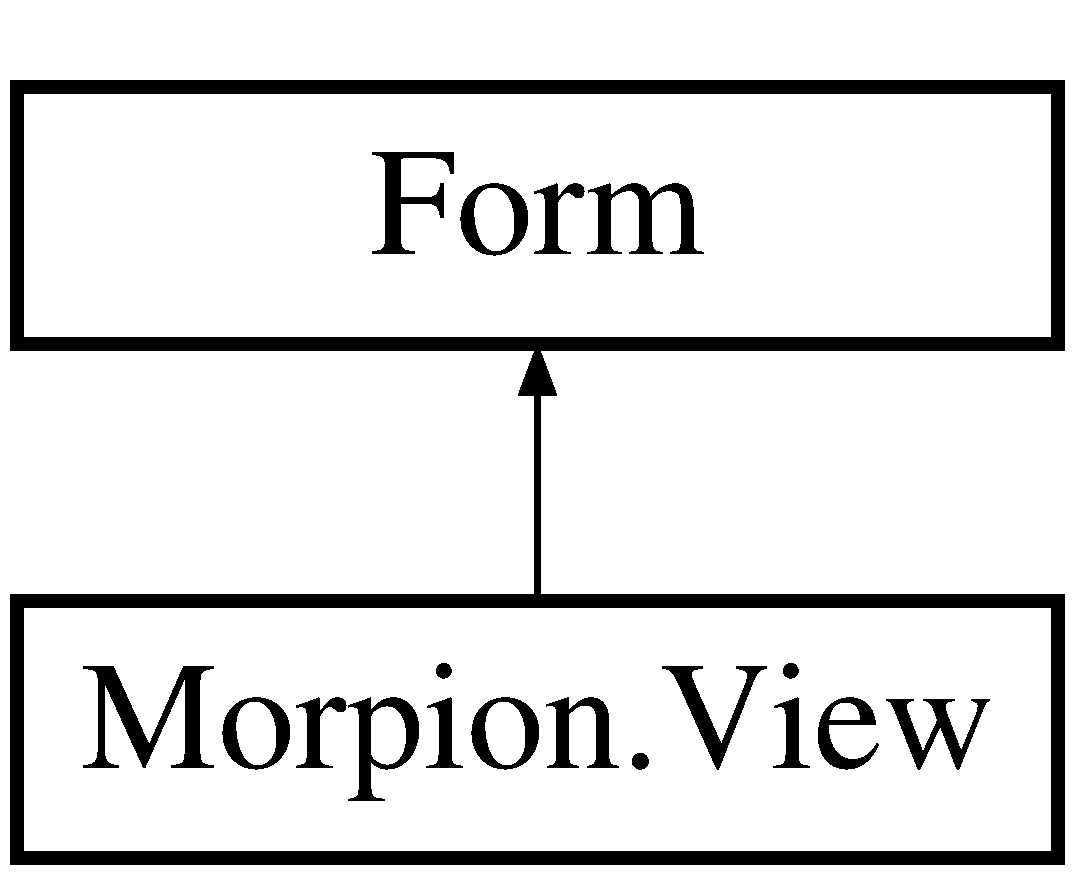
\includegraphics[height=2.000000cm]{class_morpion_1_1_view}
\end{center}
\end{figure}
\subsection*{Public Member Functions}
\begin{DoxyCompactItemize}
\item 
\hyperlink{class_morpion_1_1_view_ab8a0a6c6141f31f7e175ba5ad49140c3}{View} (string text=\char`\"{}View\char`\"{}, string name=\char`\"{}frm\+View\char`\"{})
\begin{DoxyCompactList}\small\item\em Define the name and the texte of form and disable the maximize box. \end{DoxyCompactList}\end{DoxyCompactItemize}
\subsection*{Protected Member Functions}
\begin{DoxyCompactItemize}
\item 
override void \hyperlink{class_morpion_1_1_view_a3c537c54a79236b4cfd9e78415dd48f5}{Dispose} (bool disposing)
\begin{DoxyCompactList}\small\item\em Clean up any resources being used. \end{DoxyCompactList}\end{DoxyCompactItemize}


\subsection{Detailed Description}
The form Contain all views of game 

Form view, allows the display of the different interfaces 

\subsection{Constructor \& Destructor Documentation}
\mbox{\Hypertarget{class_morpion_1_1_view_ab8a0a6c6141f31f7e175ba5ad49140c3}\label{class_morpion_1_1_view_ab8a0a6c6141f31f7e175ba5ad49140c3}} 
\index{Morpion\+::\+View@{Morpion\+::\+View}!View@{View}}
\index{View@{View}!Morpion\+::\+View@{Morpion\+::\+View}}
\subsubsection{\texorpdfstring{View()}{View()}}
{\footnotesize\ttfamily Morpion.\+View.\+View (\begin{DoxyParamCaption}\item[{string}]{text = {\ttfamily \char`\"{}View\char`\"{}},  }\item[{string}]{name = {\ttfamily \char`\"{}frmView\char`\"{}} }\end{DoxyParamCaption})}



Define the name and the texte of form and disable the maximize box. 



\subsection{Member Function Documentation}
\mbox{\Hypertarget{class_morpion_1_1_view_a3c537c54a79236b4cfd9e78415dd48f5}\label{class_morpion_1_1_view_a3c537c54a79236b4cfd9e78415dd48f5}} 
\index{Morpion\+::\+View@{Morpion\+::\+View}!Dispose@{Dispose}}
\index{Dispose@{Dispose}!Morpion\+::\+View@{Morpion\+::\+View}}
\subsubsection{\texorpdfstring{Dispose()}{Dispose()}}
{\footnotesize\ttfamily override void Morpion.\+View.\+Dispose (\begin{DoxyParamCaption}\item[{bool}]{disposing }\end{DoxyParamCaption})\hspace{0.3cm}{\ttfamily [protected]}}



Clean up any resources being used. 


\begin{DoxyParams}{Parameters}
{\em disposing} & true if managed resources should be disposed; otherwise, false.\\
\hline
\end{DoxyParams}


The documentation for this class was generated from the following files\+:\begin{DoxyCompactItemize}
\item 
C\+:/\+Users/\+Diogo.\+V\+I\+E\+I\+R\+A-\/\+F\+E\+R\+R\+E\+I\+R/\+One\+Drive -\/ C\+P\+N\+V/pre-\/tpi/\+Morpion\+\_\+\+Pre-\/\+T\+P\+I/\+C\+O\+D\+E/\+Morpion/\+Morpion/\hyperlink{_view_8cs}{View.\+cs}\item 
C\+:/\+Users/\+Diogo.\+V\+I\+E\+I\+R\+A-\/\+F\+E\+R\+R\+E\+I\+R/\+One\+Drive -\/ C\+P\+N\+V/pre-\/tpi/\+Morpion\+\_\+\+Pre-\/\+T\+P\+I/\+C\+O\+D\+E/\+Morpion/\+Morpion/\hyperlink{_view_8_designer_8cs}{View.\+Designer.\+cs}\end{DoxyCompactItemize}

\chapter{File Documentation}
\hypertarget{_controlor_8cs}{}\section{C\+:/\+Users/\+Diogo.V\+I\+E\+I\+R\+A-\/\+F\+E\+R\+R\+E\+I\+R/\+One\+Drive -\/ C\+P\+N\+V/pre-\/tpi/\+Morpion\+\_\+\+Pre-\/\+T\+P\+I/\+C\+O\+D\+E/\+Morpion/\+Morpion/\+Controlor.cs File Reference}
\label{_controlor_8cs}\index{C\+:/\+Users/\+Diogo.\+V\+I\+E\+I\+R\+A-\/\+F\+E\+R\+R\+E\+I\+R/\+One\+Drive -\/ C\+P\+N\+V/pre-\/tpi/\+Morpion\+\_\+\+Pre-\/\+T\+P\+I/\+C\+O\+D\+E/\+Morpion/\+Morpion/\+Controlor.\+cs@{C\+:/\+Users/\+Diogo.\+V\+I\+E\+I\+R\+A-\/\+F\+E\+R\+R\+E\+I\+R/\+One\+Drive -\/ C\+P\+N\+V/pre-\/tpi/\+Morpion\+\_\+\+Pre-\/\+T\+P\+I/\+C\+O\+D\+E/\+Morpion/\+Morpion/\+Controlor.\+cs}}
\subsection*{Classes}
\begin{DoxyCompactItemize}
\item 
class \hyperlink{class_morpion_1_1_controlor}{Morpion.\+Controlor}
\begin{DoxyCompactList}\small\item\em \hyperlink{class_morpion_1_1_controlor}{Controlor} manage the application. To access data, controlor call model and ask specific data. when it has data, he send to view. \end{DoxyCompactList}\end{DoxyCompactItemize}
\subsection*{Namespaces}
\begin{DoxyCompactItemize}
\item 
namespace \hyperlink{namespace_morpion}{Morpion}
\end{DoxyCompactItemize}

\hypertarget{_data_base_8cs}{}\section{C\+O\+D\+E/\+Morpion/\+Morpion/\+Data\+Base.cs File Reference}
\label{_data_base_8cs}\index{C\+O\+D\+E/\+Morpion/\+Morpion/\+Data\+Base.\+cs@{C\+O\+D\+E/\+Morpion/\+Morpion/\+Data\+Base.\+cs}}
\subsection*{Classes}
\begin{DoxyCompactItemize}
\item 
class \hyperlink{class_morpion_1_1_data_base}{Morpion.\+Data\+Base}
\begin{DoxyCompactList}\small\item\em The class give access to DB \end{DoxyCompactList}\end{DoxyCompactItemize}
\subsection*{Namespaces}
\begin{DoxyCompactItemize}
\item 
namespace \hyperlink{namespace_morpion}{Morpion}
\end{DoxyCompactItemize}

\hypertarget{_model_8cs}{}\section{C\+O\+D\+E/\+Morpion/\+Morpion/\+Model.cs File Reference}
\label{_model_8cs}\index{C\+O\+D\+E/\+Morpion/\+Morpion/\+Model.\+cs@{C\+O\+D\+E/\+Morpion/\+Morpion/\+Model.\+cs}}
\subsection*{Classes}
\begin{DoxyCompactItemize}
\item 
class \hyperlink{class_morpion_1_1_model}{Morpion.\+Model}
\end{DoxyCompactItemize}
\subsection*{Namespaces}
\begin{DoxyCompactItemize}
\item 
namespace \hyperlink{namespace_morpion}{Morpion}
\end{DoxyCompactItemize}

\hypertarget{_network_communication_8cs}{}\section{C\+:/\+Users/\+Diogo.V\+I\+E\+I\+R\+A-\/\+F\+E\+R\+R\+E\+I\+R/\+One\+Drive -\/ C\+P\+N\+V/pre-\/tpi/\+Morpion\+\_\+\+Pre-\/\+T\+P\+I/\+C\+O\+D\+E/\+Morpion/\+Morpion/\+Network\+Communication.cs File Reference}
\label{_network_communication_8cs}\index{C\+:/\+Users/\+Diogo.\+V\+I\+E\+I\+R\+A-\/\+F\+E\+R\+R\+E\+I\+R/\+One\+Drive -\/ C\+P\+N\+V/pre-\/tpi/\+Morpion\+\_\+\+Pre-\/\+T\+P\+I/\+C\+O\+D\+E/\+Morpion/\+Morpion/\+Network\+Communication.\+cs@{C\+:/\+Users/\+Diogo.\+V\+I\+E\+I\+R\+A-\/\+F\+E\+R\+R\+E\+I\+R/\+One\+Drive -\/ C\+P\+N\+V/pre-\/tpi/\+Morpion\+\_\+\+Pre-\/\+T\+P\+I/\+C\+O\+D\+E/\+Morpion/\+Morpion/\+Network\+Communication.\+cs}}
\subsection*{Classes}
\begin{DoxyCompactItemize}
\item 
class \hyperlink{class_morpion_1_1_network_communication}{Morpion.\+Network\+Communication}
\end{DoxyCompactItemize}
\subsection*{Namespaces}
\begin{DoxyCompactItemize}
\item 
namespace \hyperlink{namespace_morpion}{Morpion}
\end{DoxyCompactItemize}

\hypertarget{_morpion_2obj_2_debug_2_temporary_generated_file__036_c0_b5_b-1481-4323-8_d20-8_f5_a_d_c_b23_d92_8cs}{}\section{C\+O\+D\+E/\+Morpion/\+Morpion/obj/\+Debug/\+Temporary\+Generated\+File\+\_\+036\+C0\+B5\+B-\/1481-\/4323-\/8\+D20-\/8\+F5\+A\+D\+C\+B23\+D92.cs File Reference}
\label{_morpion_2obj_2_debug_2_temporary_generated_file__036_c0_b5_b-1481-4323-8_d20-8_f5_a_d_c_b23_d92_8cs}\index{C\+O\+D\+E/\+Morpion/\+Morpion/obj/\+Debug/\+Temporary\+Generated\+File\+\_\+036\+C0\+B5\+B-\/1481-\/4323-\/8\+D20-\/8\+F5\+A\+D\+C\+B23\+D92.\+cs@{C\+O\+D\+E/\+Morpion/\+Morpion/obj/\+Debug/\+Temporary\+Generated\+File\+\_\+036\+C0\+B5\+B-\/1481-\/4323-\/8\+D20-\/8\+F5\+A\+D\+C\+B23\+D92.\+cs}}

\hypertarget{_test_morpion_2obj_2_debug_2_temporary_generated_file__036_c0_b5_b-1481-4323-8_d20-8_f5_a_d_c_b23_d92_8cs}{}\section{C\+:/\+Users/\+Diogo.V\+I\+E\+I\+R\+A-\/\+F\+E\+R\+R\+E\+I\+R/\+One\+Drive -\/ C\+P\+N\+V/pre-\/tpi/\+Morpion\+\_\+\+Pre-\/\+T\+P\+I/\+C\+O\+D\+E/\+Morpion/\+Test\+Morpion/obj/\+Debug/\+Temporary\+Generated\+File\+\_\+036\+C0\+B5\+B-\/1481-\/4323-\/8\+D20-\/8\+F5\+A\+D\+C\+B23\+D92.cs File Reference}
\label{_test_morpion_2obj_2_debug_2_temporary_generated_file__036_c0_b5_b-1481-4323-8_d20-8_f5_a_d_c_b23_d92_8cs}\index{C\+:/\+Users/\+Diogo.\+V\+I\+E\+I\+R\+A-\/\+F\+E\+R\+R\+E\+I\+R/\+One\+Drive -\/ C\+P\+N\+V/pre-\/tpi/\+Morpion\+\_\+\+Pre-\/\+T\+P\+I/\+C\+O\+D\+E/\+Morpion/\+Test\+Morpion/obj/\+Debug/\+Temporary\+Generated\+File\+\_\+036\+C0\+B5\+B-\/1481-\/4323-\/8\+D20-\/8\+F5\+A\+D\+C\+B23\+D92.\+cs@{C\+:/\+Users/\+Diogo.\+V\+I\+E\+I\+R\+A-\/\+F\+E\+R\+R\+E\+I\+R/\+One\+Drive -\/ C\+P\+N\+V/pre-\/tpi/\+Morpion\+\_\+\+Pre-\/\+T\+P\+I/\+C\+O\+D\+E/\+Morpion/\+Test\+Morpion/obj/\+Debug/\+Temporary\+Generated\+File\+\_\+036\+C0\+B5\+B-\/1481-\/4323-\/8\+D20-\/8\+F5\+A\+D\+C\+B23\+D92.\+cs}}

\hypertarget{_morpion_2obj_2_debug_2_temporary_generated_file__5937a670-0e60-4077-877b-f7221da3dda1_8cs}{}\section{C\+:/\+Users/\+Diogo.V\+I\+E\+I\+R\+A-\/\+F\+E\+R\+R\+E\+I\+R/\+One\+Drive -\/ C\+P\+N\+V/pre-\/tpi/\+Morpion\+\_\+\+Pre-\/\+T\+P\+I/\+C\+O\+D\+E/\+Morpion/\+Morpion/obj/\+Debug/\+Temporary\+Generated\+File\+\_\+5937a670-\/0e60-\/4077-\/877b-\/f7221da3dda1.cs File Reference}
\label{_morpion_2obj_2_debug_2_temporary_generated_file__5937a670-0e60-4077-877b-f7221da3dda1_8cs}\index{C\+:/\+Users/\+Diogo.\+V\+I\+E\+I\+R\+A-\/\+F\+E\+R\+R\+E\+I\+R/\+One\+Drive -\/ C\+P\+N\+V/pre-\/tpi/\+Morpion\+\_\+\+Pre-\/\+T\+P\+I/\+C\+O\+D\+E/\+Morpion/\+Morpion/obj/\+Debug/\+Temporary\+Generated\+File\+\_\+5937a670-\/0e60-\/4077-\/877b-\/f7221da3dda1.\+cs@{C\+:/\+Users/\+Diogo.\+V\+I\+E\+I\+R\+A-\/\+F\+E\+R\+R\+E\+I\+R/\+One\+Drive -\/ C\+P\+N\+V/pre-\/tpi/\+Morpion\+\_\+\+Pre-\/\+T\+P\+I/\+C\+O\+D\+E/\+Morpion/\+Morpion/obj/\+Debug/\+Temporary\+Generated\+File\+\_\+5937a670-\/0e60-\/4077-\/877b-\/f7221da3dda1.\+cs}}

\hypertarget{_test_morpion_2obj_2_debug_2_temporary_generated_file__5937a670-0e60-4077-877b-f7221da3dda1_8cs}{}\section{C\+O\+D\+E/\+Morpion/\+Test\+Morpion/obj/\+Debug/\+Temporary\+Generated\+File\+\_\+5937a670-\/0e60-\/4077-\/877b-\/f7221da3dda1.cs File Reference}
\label{_test_morpion_2obj_2_debug_2_temporary_generated_file__5937a670-0e60-4077-877b-f7221da3dda1_8cs}\index{C\+O\+D\+E/\+Morpion/\+Test\+Morpion/obj/\+Debug/\+Temporary\+Generated\+File\+\_\+5937a670-\/0e60-\/4077-\/877b-\/f7221da3dda1.\+cs@{C\+O\+D\+E/\+Morpion/\+Test\+Morpion/obj/\+Debug/\+Temporary\+Generated\+File\+\_\+5937a670-\/0e60-\/4077-\/877b-\/f7221da3dda1.\+cs}}

\hypertarget{_morpion_2obj_2_debug_2_temporary_generated_file___e7_a71_f73-0_f8_d-4_b9_b-_b56_e-8_e70_b10_b_c5_d3_8cs}{}\section{C\+O\+D\+E/\+Morpion/\+Morpion/obj/\+Debug/\+Temporary\+Generated\+File\+\_\+\+E7\+A71\+F73-\/0\+F8\+D-\/4\+B9\+B-\/\+B56\+E-\/8\+E70\+B10\+B\+C5\+D3.cs File Reference}
\label{_morpion_2obj_2_debug_2_temporary_generated_file___e7_a71_f73-0_f8_d-4_b9_b-_b56_e-8_e70_b10_b_c5_d3_8cs}\index{C\+O\+D\+E/\+Morpion/\+Morpion/obj/\+Debug/\+Temporary\+Generated\+File\+\_\+\+E7\+A71\+F73-\/0\+F8\+D-\/4\+B9\+B-\/\+B56\+E-\/8\+E70\+B10\+B\+C5\+D3.\+cs@{C\+O\+D\+E/\+Morpion/\+Morpion/obj/\+Debug/\+Temporary\+Generated\+File\+\_\+\+E7\+A71\+F73-\/0\+F8\+D-\/4\+B9\+B-\/\+B56\+E-\/8\+E70\+B10\+B\+C5\+D3.\+cs}}

\hypertarget{_test_morpion_2obj_2_debug_2_temporary_generated_file___e7_a71_f73-0_f8_d-4_b9_b-_b56_e-8_e70_b10_b_c5_d3_8cs}{}\section{C\+:/\+Users/\+Diogo.V\+I\+E\+I\+R\+A-\/\+F\+E\+R\+R\+E\+I\+R/\+One\+Drive -\/ C\+P\+N\+V/pre-\/tpi/\+Morpion\+\_\+\+Pre-\/\+T\+P\+I/\+C\+O\+D\+E/\+Morpion/\+Test\+Morpion/obj/\+Debug/\+Temporary\+Generated\+File\+\_\+\+E7\+A71\+F73-\/0\+F8\+D-\/4\+B9\+B-\/\+B56\+E-\/8\+E70\+B10\+B\+C5\+D3.cs File Reference}
\label{_test_morpion_2obj_2_debug_2_temporary_generated_file___e7_a71_f73-0_f8_d-4_b9_b-_b56_e-8_e70_b10_b_c5_d3_8cs}\index{C\+:/\+Users/\+Diogo.\+V\+I\+E\+I\+R\+A-\/\+F\+E\+R\+R\+E\+I\+R/\+One\+Drive -\/ C\+P\+N\+V/pre-\/tpi/\+Morpion\+\_\+\+Pre-\/\+T\+P\+I/\+C\+O\+D\+E/\+Morpion/\+Test\+Morpion/obj/\+Debug/\+Temporary\+Generated\+File\+\_\+\+E7\+A71\+F73-\/0\+F8\+D-\/4\+B9\+B-\/\+B56\+E-\/8\+E70\+B10\+B\+C5\+D3.\+cs@{C\+:/\+Users/\+Diogo.\+V\+I\+E\+I\+R\+A-\/\+F\+E\+R\+R\+E\+I\+R/\+One\+Drive -\/ C\+P\+N\+V/pre-\/tpi/\+Morpion\+\_\+\+Pre-\/\+T\+P\+I/\+C\+O\+D\+E/\+Morpion/\+Test\+Morpion/obj/\+Debug/\+Temporary\+Generated\+File\+\_\+\+E7\+A71\+F73-\/0\+F8\+D-\/4\+B9\+B-\/\+B56\+E-\/8\+E70\+B10\+B\+C5\+D3.\+cs}}

\hypertarget{_program_8cs}{}\section{C\+O\+D\+E/\+Morpion/\+Morpion/\+Program.cs File Reference}
\label{_program_8cs}\index{C\+O\+D\+E/\+Morpion/\+Morpion/\+Program.\+cs@{C\+O\+D\+E/\+Morpion/\+Morpion/\+Program.\+cs}}
\subsection*{Classes}
\begin{DoxyCompactItemize}
\item 
class {\bfseries Morpion.\+Program}
\end{DoxyCompactItemize}
\subsection*{Namespaces}
\begin{DoxyCompactItemize}
\item 
namespace \hyperlink{namespace_morpion}{Morpion}
\end{DoxyCompactItemize}

\hypertarget{_morpion_2_properties_2_assembly_info_8cs}{}\section{C\+O\+D\+E/\+Morpion/\+Morpion/\+Properties/\+Assembly\+Info.cs File Reference}
\label{_morpion_2_properties_2_assembly_info_8cs}\index{C\+O\+D\+E/\+Morpion/\+Morpion/\+Properties/\+Assembly\+Info.\+cs@{C\+O\+D\+E/\+Morpion/\+Morpion/\+Properties/\+Assembly\+Info.\+cs}}

\hypertarget{_test_morpion_2_properties_2_assembly_info_8cs}{}\section{C\+O\+D\+E/\+Morpion/\+Test\+Morpion/\+Properties/\+Assembly\+Info.cs File Reference}
\label{_test_morpion_2_properties_2_assembly_info_8cs}\index{C\+O\+D\+E/\+Morpion/\+Test\+Morpion/\+Properties/\+Assembly\+Info.\+cs@{C\+O\+D\+E/\+Morpion/\+Test\+Morpion/\+Properties/\+Assembly\+Info.\+cs}}

\hypertarget{_resources_8_designer_8cs}{}\section{C\+O\+D\+E/\+Morpion/\+Morpion/\+Properties/\+Resources.Designer.\+cs File Reference}
\label{_resources_8_designer_8cs}\index{C\+O\+D\+E/\+Morpion/\+Morpion/\+Properties/\+Resources.\+Designer.\+cs@{C\+O\+D\+E/\+Morpion/\+Morpion/\+Properties/\+Resources.\+Designer.\+cs}}
\subsection*{Classes}
\begin{DoxyCompactItemize}
\item 
class {\bfseries Morpion.\+Properties.\+Resources}
\begin{DoxyCompactList}\small\item\em A strongly-\/typed resource class, for looking up localized strings, etc. \end{DoxyCompactList}\end{DoxyCompactItemize}
\subsection*{Namespaces}
\begin{DoxyCompactItemize}
\item 
namespace \hyperlink{namespace_morpion_1_1_properties}{Morpion.\+Properties}
\end{DoxyCompactItemize}

\hypertarget{_settings_8_designer_8cs}{}\section{C\+O\+D\+E/\+Morpion/\+Morpion/\+Properties/\+Settings.Designer.\+cs File Reference}
\label{_settings_8_designer_8cs}\index{C\+O\+D\+E/\+Morpion/\+Morpion/\+Properties/\+Settings.\+Designer.\+cs@{C\+O\+D\+E/\+Morpion/\+Morpion/\+Properties/\+Settings.\+Designer.\+cs}}
\subsection*{Classes}
\begin{DoxyCompactItemize}
\item 
class {\bfseries Morpion.\+Properties.\+Settings}
\end{DoxyCompactItemize}
\subsection*{Namespaces}
\begin{DoxyCompactItemize}
\item 
namespace \hyperlink{namespace_morpion_1_1_properties}{Morpion.\+Properties}
\end{DoxyCompactItemize}

\hypertarget{score_8cs}{}\section{C\+:/\+Users/\+Diogo.V\+I\+E\+I\+R\+A-\/\+F\+E\+R\+R\+E\+I\+R/\+One\+Drive -\/ C\+P\+N\+V/pre-\/tpi/\+Morpion\+\_\+\+Pre-\/\+T\+P\+I/\+C\+O\+D\+E/\+Morpion/\+Morpion/score.cs File Reference}
\label{score_8cs}\index{C\+:/\+Users/\+Diogo.\+V\+I\+E\+I\+R\+A-\/\+F\+E\+R\+R\+E\+I\+R/\+One\+Drive -\/ C\+P\+N\+V/pre-\/tpi/\+Morpion\+\_\+\+Pre-\/\+T\+P\+I/\+C\+O\+D\+E/\+Morpion/\+Morpion/score.\+cs@{C\+:/\+Users/\+Diogo.\+V\+I\+E\+I\+R\+A-\/\+F\+E\+R\+R\+E\+I\+R/\+One\+Drive -\/ C\+P\+N\+V/pre-\/tpi/\+Morpion\+\_\+\+Pre-\/\+T\+P\+I/\+C\+O\+D\+E/\+Morpion/\+Morpion/score.\+cs}}
\subsection*{Classes}
\begin{DoxyCompactItemize}
\item 
class \hyperlink{class_morpion_1_1score}{Morpion.\+score}
\begin{DoxyCompactList}\small\item\em this class allows to create an object containing the score between 2 players \end{DoxyCompactList}\end{DoxyCompactItemize}
\subsection*{Namespaces}
\begin{DoxyCompactItemize}
\item 
namespace \hyperlink{namespace_morpion}{Morpion}
\end{DoxyCompactItemize}

\hypertarget{_view_8cs}{}\section{C\+:/\+Users/\+Diogo.V\+I\+E\+I\+R\+A-\/\+F\+E\+R\+R\+E\+I\+R/\+One\+Drive -\/ C\+P\+N\+V/pre-\/tpi/\+Morpion\+\_\+\+Pre-\/\+T\+P\+I/\+C\+O\+D\+E/\+Morpion/\+Morpion/\+View.cs File Reference}
\label{_view_8cs}\index{C\+:/\+Users/\+Diogo.\+V\+I\+E\+I\+R\+A-\/\+F\+E\+R\+R\+E\+I\+R/\+One\+Drive -\/ C\+P\+N\+V/pre-\/tpi/\+Morpion\+\_\+\+Pre-\/\+T\+P\+I/\+C\+O\+D\+E/\+Morpion/\+Morpion/\+View.\+cs@{C\+:/\+Users/\+Diogo.\+V\+I\+E\+I\+R\+A-\/\+F\+E\+R\+R\+E\+I\+R/\+One\+Drive -\/ C\+P\+N\+V/pre-\/tpi/\+Morpion\+\_\+\+Pre-\/\+T\+P\+I/\+C\+O\+D\+E/\+Morpion/\+Morpion/\+View.\+cs}}
\subsection*{Classes}
\begin{DoxyCompactItemize}
\item 
class \hyperlink{class_morpion_1_1_view}{Morpion.\+View}
\begin{DoxyCompactList}\small\item\em The form Contain all views of game \end{DoxyCompactList}\end{DoxyCompactItemize}
\subsection*{Namespaces}
\begin{DoxyCompactItemize}
\item 
namespace \hyperlink{namespace_morpion}{Morpion}
\end{DoxyCompactItemize}

\hypertarget{_view_8_designer_8cs}{}\section{C\+:/\+Users/\+Diogo.V\+I\+E\+I\+R\+A-\/\+F\+E\+R\+R\+E\+I\+R/\+One\+Drive -\/ C\+P\+N\+V/pre-\/tpi/\+Morpion\+\_\+\+Pre-\/\+T\+P\+I/\+C\+O\+D\+E/\+Morpion/\+Morpion/\+View.Designer.\+cs File Reference}
\label{_view_8_designer_8cs}\index{C\+:/\+Users/\+Diogo.\+V\+I\+E\+I\+R\+A-\/\+F\+E\+R\+R\+E\+I\+R/\+One\+Drive -\/ C\+P\+N\+V/pre-\/tpi/\+Morpion\+\_\+\+Pre-\/\+T\+P\+I/\+C\+O\+D\+E/\+Morpion/\+Morpion/\+View.\+Designer.\+cs@{C\+:/\+Users/\+Diogo.\+V\+I\+E\+I\+R\+A-\/\+F\+E\+R\+R\+E\+I\+R/\+One\+Drive -\/ C\+P\+N\+V/pre-\/tpi/\+Morpion\+\_\+\+Pre-\/\+T\+P\+I/\+C\+O\+D\+E/\+Morpion/\+Morpion/\+View.\+Designer.\+cs}}
\subsection*{Classes}
\begin{DoxyCompactItemize}
\item 
class \hyperlink{class_morpion_1_1_view}{Morpion.\+View}
\begin{DoxyCompactList}\small\item\em The form Contain all views of game \end{DoxyCompactList}\end{DoxyCompactItemize}
\subsection*{Namespaces}
\begin{DoxyCompactItemize}
\item 
namespace \hyperlink{namespace_morpion}{Morpion}
\end{DoxyCompactItemize}

\hypertarget{_test_d_b_8cs}{}\section{C\+O\+D\+E/\+Morpion/\+Test\+Morpion/\+Test\+DB.cs File Reference}
\label{_test_d_b_8cs}\index{C\+O\+D\+E/\+Morpion/\+Test\+Morpion/\+Test\+D\+B.\+cs@{C\+O\+D\+E/\+Morpion/\+Test\+Morpion/\+Test\+D\+B.\+cs}}
\subsection*{Classes}
\begin{DoxyCompactItemize}
\item 
class \hyperlink{class_test_morpion_1_1_test_d_b}{Test\+Morpion.\+Test\+DB}
\end{DoxyCompactItemize}
\subsection*{Namespaces}
\begin{DoxyCompactItemize}
\item 
namespace \hyperlink{namespace_test_morpion}{Test\+Morpion}
\end{DoxyCompactItemize}

\hypertarget{_test_model_8cs}{}\section{C\+:/\+Users/\+Diogo.V\+I\+E\+I\+R\+A-\/\+F\+E\+R\+R\+E\+I\+R/\+One\+Drive -\/ C\+P\+N\+V/pre-\/tpi/\+Morpion\+\_\+\+Pre-\/\+T\+P\+I/\+C\+O\+D\+E/\+Morpion/\+Test\+Morpion/\+Test\+Model.cs File Reference}
\label{_test_model_8cs}\index{C\+:/\+Users/\+Diogo.\+V\+I\+E\+I\+R\+A-\/\+F\+E\+R\+R\+E\+I\+R/\+One\+Drive -\/ C\+P\+N\+V/pre-\/tpi/\+Morpion\+\_\+\+Pre-\/\+T\+P\+I/\+C\+O\+D\+E/\+Morpion/\+Test\+Morpion/\+Test\+Model.\+cs@{C\+:/\+Users/\+Diogo.\+V\+I\+E\+I\+R\+A-\/\+F\+E\+R\+R\+E\+I\+R/\+One\+Drive -\/ C\+P\+N\+V/pre-\/tpi/\+Morpion\+\_\+\+Pre-\/\+T\+P\+I/\+C\+O\+D\+E/\+Morpion/\+Test\+Morpion/\+Test\+Model.\+cs}}
\subsection*{Classes}
\begin{DoxyCompactItemize}
\item 
class \hyperlink{class_test_morpion_1_1_test_model}{Test\+Morpion.\+Test\+Model}
\end{DoxyCompactItemize}
\subsection*{Namespaces}
\begin{DoxyCompactItemize}
\item 
namespace \hyperlink{namespace_test_morpion}{Test\+Morpion}
\end{DoxyCompactItemize}

%--- End generated contents ---

% Index
\backmatter
\newpage
\phantomsection
\clearemptydoublepage
\addcontentsline{toc}{chapter}{Index}
\printindex

\end{document}
